\documentclass[12pt,a4paper,openright,twoside]{book}
\usepackage[utf8]{inputenc}
\usepackage[english, italian]{babel}
\usepackage{disi-thesis}
\usepackage{code-lstlistings}
\usepackage{notes}
\usepackage{shortcuts}
\usepackage{acronym}
\usepackage{listings}
\usepackage{xcolor}
\usepackage{tikz}
\usepackage{array}   
\usepackage{float}
\usepackage{booktabs}
\usepackage{longtable}
\newcolumntype{L}[1]{>{\raggedright\arraybackslash}p{#1}}

\lstdefinelanguage{json}{
    basicstyle=\footnotesize\ttfamily,numbers=none,breaklines=true,
    frame=lines,backgroundcolor=\color{gray!10},showstringspaces=false,
    string=[db]{"},stringstyle=\color{green!50!black},
    morestring=[s][\color{black}]{\ \ "}{":},keywordstyle=\color{blue},
    keywords={true,false,null},literate=*{0}{{{\color{red}0}}}{1}
    {1}{{{\color{red}1}}}{1}{2}{{{\color{red}2}}}{1}{3}{{{\color{red}3}}}{1}
    {4}{{{\color{red}4}}}{1}{5}{{{\color{red}5}}}{1}{6}{{{\color{red}6}}}{1}
    {7}{{{\color{red}7}}}{1}{8}{{{\color{red}8}}}{1}{9}{{{\color{red}9}}}{1}
    {.}{{{\color{red}.}}}{1}{:}{{{\color{gray}{:}}}}{1}{,}{{{\color{gray}{,}}}}{1}
    {\{}{{{\color{gray}{\{}}}}{1}{\}}{{{\color{gray}{\}}}}}{1}{[}{{{\color{gray}{[}}}}{1}{]}{{{\color{gray}{]}}}}{1}
}

\usetikzlibrary{shapes,arrows,positioning}
\usetikzlibrary{fit}
\usetikzlibrary{calc}
\tikzstyle{block} = [rectangle, draw, fill=white, 
    text width=3cm, text centered, rounded corners, minimum height=2em]
\tikzstyle{line} = [draw, -latex']

\school{\unibo}
\programme{Corso di Laurea in Ingegneria e Scienze Informatiche}
\title{Integrazione di RAG e LLM nello Sviluppo del Software}
\author{Bollini Simone}
\date{\today}
\subject{Programmazione ad oggetti}
\supervisor{Prof. Viroli Mirko}
\cosupervisor{Dott. Aguzzi Gianluca}
%\morecosupervisor{Dott. Farabegoli Nicolas}
\session{IV}
\academicyear{2023-2024}

% Definition of acronyms
\acrodef{RAG}{Retrieval-Augmented Generation}
\acrodef{AI}{Artificial intelligence}
\acrodef{LLM}{Large Language Model}


\mainlinespacing{1.241} % line spacing in mainmatter, comment to default (1)

\begin{document}
\frontmatter\frontispiece
\begin{abstract}	
I \ac{LLM} addestrati per sviluppare il codice sono oggi altamente efficaci e in grado di generare soluzioni di qualità.
Ma l'addestramento fatto sui modelli è su fonti generali, questo non da quindi la possibilità al modello di generare soluzioni su misura per una specifica richiesta partendo da codice già creato dal programmatore o dalla propria azienda per casi simili.
Da questo nasce l'esigenza di addestrare il modello per personalizzare le soluzioni proposte, contestualizzandole alla propria realtà aziendale e al proprio stile nel programmare.
Servirebbe quindi una nuova fase di fine-tunig per adattare il modello alle proprie esigenze, ma questa soluzione è un processo molto costoso che richiede particolari competenze tecnica
difficilmente presenti in molte aziende. Inoltre il fine-tuning non permette di aggiornare il modello in maniera rapida e dinamica, richiedendo un nuovo addestramento per ogni modifica.
Per rispondere a questa esigenza entra in gioco la \ac{RAG}, che permette di aumentare la conoscenza del modello, recuperando informazioni da una propria base di conoscenza arricchendo il prompt della query di input che sarà elaborata dal \ac{LLM}.
Il \ac{RAG}, ricercando semanticamente i chunk maggiormente somiglianti a quanto richiesto se trovati, li inserirà per aumentare il Prompt del LLM, estendendo la base di informazioni sulla quale genererà l'output con la risposta.
Questa tesi approfondisce questi concetti e sperimenta l'integrazione di un \ac{RAG} specifico per codice Java e un \ac{LLM} con lo scopo di ottenere risposte personalizzate
che solo con la conoscenza del LLM, anche se estremamente performante e completo, sarebbe stato impossibile ottenere.
\end{abstract}

\begin{dedication}
A Giulia e ai miei figli, il dono più incredibile di questa vita.
\newline Alla mia grande famiglia.
\newline Grazie
\end{dedication}

%----------------------------------------------------------------------------------------
\tableofcontents   
%\listoffigures     % (optional) comment if empty
%\lstlistoflistings % (optional) comment if empty
%----------------------------------------------------------------------------------------

\mainmatter

%----------------------------------------------------------------------------------------
\chapter{Introduzione}
\label{chap:introduction}
%----------------------------------------------------------------------------------------
Il mondo della programmazione è un settore in continua evoluzione e negli ultimi anni ha visto un esplosione nel campo dell'\ac{AI}.
Con l'avvento di questa nuova tecnologia per molti programmatori è cambiato il modo di lavorare, utilizzando come assistenti durante la produzione del codice software basati sull'\ac{AI}.
Questi software sono in grado di completare il codice, debugging, suggerire correzioni e creare documentazione pertinente.
Aiutano inoltre i programmatori nei compiti più ripetivi e meccanici, aumentando la produttività e riducendo i tempi di sviluppo.
Ad esempio in \textbf{Github Copilot} che è un assistente per la scrittura del codice, basato su \ac{LLM}, è presenta il comando: \emph{'Generate Commit Message with Copilot'}
che propone il testo da utilizzare come descrizione di un commit, basandosi sulle modifiche apportate al codice come mostrato in figura \cref{fig:Commit-Autogenerato}.
\begin{figure}[h]
    \centering
    \includegraphics[width=0.5\linewidth]{figures/commit.png}
    \caption{Esempio di commit autogenerato da Copilot}
    \label{fig:Commit-Autogenerato}
\end{figure}

Software come Copilot utilizzano LLM per riprodurre codice e testo, scansionando in pochi istanti il contesto nel codice che si sta costruendo.
In progetti complessi questo non riduce il ruolo del programmatore che detiene la realizzazione di compiti complessi ad alto valore aggiunto delegando la generazione di parti del codice semplici e ripetitive a questi software.
\`E quindi importante capire il funzionamento di questi strumenti, sapere come chiedere e formulare correttamente le domande, esplicitando nel dettaglio con parole chiave mirate come deve essere realizzato il codice per indizzare il \ac{LLM} nell'elaborazione e ragionamento corretto.
\begin{figure}[h]
    \centering
    \includegraphics[width=0.5\linewidth]{figures/copilotsolutionSettimanaEnigmistica.png}
    \caption{Copilot scansionando il codice spesso trova valide soluzioni}
    \label{fig:Copilot-Solution}
\end{figure}
Questi software hanno un problema importante, essendo addestrati su dataset generici e non personalizzati, sono validi nel fornire risposte standard e generiche, ma non sono in grado di fornire risposte personalizzate e specifiche per un'azienda o un programmatore.
Proprio per questo l'ultimo miglio da percorrere per sfruttare questi strumenti è la personalizzazione delle risposte, per fare in modo che il LLM impari lo stile del programmatore e produca codice coerente con quanto già realizzato e conosciuto.
Per fare questo entrano in gioco il \textbf{Fine-Tuning} e i \textbf{RAG} che sono l'argomento principale di questa tesi.
\chapter{Addestrare un LLM per la Generazione del Codice}

L'addestramento di LLM per la generazione del codice di programmazione richiede una serie di passaggi complessi e costi significativi.
Conoscere questo processo è utile per poter poi comprendere al meglio la successiva implementazione con le tecniche di \textbf{RAG}.
La procedura si divide nelle seguenti fasi:
\begin{itemize}
    \item Scelta del Modello
    \item Raccolta e Preparazione dei Dataset
    \item Pre-Addestramento
    \item Fine-Tuning
    \item Valutazione e Ottimizzazione
\end{itemize}
Analizziamo ora nel dettaglio ogni fase.
\section{Scelta Modello}
Gli LLM utilizzano tipicamente architetture basate su transformers, che sono particolarmente efficaci nell'elaborazione di sequenze di dati, come il testo e il codice.
I transformers utilizzano meccanismi di auto-attenzione per valutare l'importanza di diversi elementi in una sequenza,
permettendo al modello di comprendere le relazioni tra parole o token.
Questa capacità è fondamentale nella generazione del codice, poiché le dipendenze tra variabili e funzioni possono estendersi su ampie sezioni del codice, richiedendo al modello di considerare un ampio contesto per trovare le risposte corrette.
L'architettura del modello scelto influenzerà in maniera decisiva tutte le successive fasi di addestramento.
È utile notare che sebbene i transformers siano attualmente lo standard, esistono anche altri approcci come le reti neurali ricorrenti (RNN e LSTM) e nuove tecniche in continua evoluzione come i Large Concept Models \cite{code-llm-survey-2024}.
\section{Raccolta e Preparazione dei Dataset}
La qualità e la quantità dei dati per l'addestramento è di primaria importanza per prepare un modello alla generazione di codice in maniera efficace.
È quindi essenziale utilizzare per il training codice proveniente da molteplici fonti tra cui codice sorgente, file readme, documentazione tecnica, commenti nel codice,
pagine Wiki, API e discussioni su forum specializzati in programmazione, arricchendo così il dataset con esempi pratici e ricchezza terminologica.
In rete è possibile trovare diverso materiale open source tra cui dataset già etichettati.
Alcuni dataset hanno un valore altissimo, per questo motivo per tutelare il costo speso per produrli per certi dataset è previsto il diritto d'autore.
I dati si dividono in due tipologie:
\begin{itemize}
    \item \textbf{Dati Strutturati}: seguono un formato specifico e predefinito, seguono la struttora in coppie (descrizione, codice).
    \item \textbf{Dati non Strutturati}: non sono organizzati e sono quindi più difficili da interpretare dal modello. 
\end{itemize}
\subsection{Pulizia e Pre-Processo}
La raccolta di dati va visionata con cura, se non si conosce la provenienza del codice è possibile che contenga bug o codice obsoleto che possono essere trasmessi al modello.
Con la rapida evoluzione del codice molte librerie e tecniche vengono \textbf{rapidamente deprecate} e superate per questo anche utilizzando i più noti modelli LLM ad oggi disponibili, può capitare di ricevere come output \textbf{codice obsoleto che risolve il quesito ma con soluzioni contenti tecniche, api e librerie deprecate o non più disponibili.}
Per questo motivo i dati raccolti devono essere puliti e pre-processati per rimuovere errori e informazioni non pertinenti, garantendo così un dataset di alta qualità per l'addestramento.
\subsubsection{Tokenizzazione}
Il modello per poter elaborare il dataset ha bisogno che quest'ultimo venga diviso in parti più piccole chiamate token per mantenere l'integrita del dato \cite{stanford-codegen},
i token possono essere parole, parti di parole o singoli caratteri, e questa suddivisione è fondamentale per:

\begin{itemize}
    \item \textbf{Gestione del contesto}: mantenere la relazione semantica tra i diversi elementi del codice
    \item \textbf{Efficienza computazionale}: processare grandi quantità di testo in modo ottimizzato
    \item \textbf{Limitazioni del modello}: rispettare i limiti massimi di input del modello (tipicamente tra 512 e 4096 token)
    \item \textbf{Preservazione della struttura}: mantenere la struttura sintattica del codice sorgente
\end{itemize}

Ad esempio, nel codice Java, i token potrebbero includere:
\begin{itemize}
    \item Parole chiave (\texttt{public}, \texttt{class}, \texttt{static})
    \item Identificatori (nomi di variabili e metodi)
    \item Operatori e simboli (\texttt{+}, \texttt{=}, \texttt{\{}, \texttt{\}})
    \item Stringhe letterali e commenti
\end{itemize}
\section{Pre-Addestramento}
Il pre-addestramento di un LLM specializzato nella generazione di codice ha lo scopo di fornire al modello una conoscenza generale della sintassi e delle strutture logiche dei linguaggio di programmazione.
Durante questa fase il modello impare a generare codice partendo da dati non etichettati utilizzando tecniche come il \emph{language modeling} autoregressivo per insegnare al modello di predire il token successivo in una sequenza.
Questo approccio rende la generazione contestualmente e coerente di codice, sfruttando la capacità del modello di 'ricordare' il contesto anche su ampie sequenze di dati.
\section{Fine-Tuning}
Il fine-tuning è la fase in cui il modello già pre-addestrato viene ulteriormente specializzato per la generazione di codice adattando e migliorando il modello per specifici domini di applicazione.
Durante questa fase, il modello affina le sue capacità attraverso dataset specializzati composti da coppie descrizione-codice, documentazione tecnica e commenti, esempi di bug-fixing e refactoring.
\subsection{Tecniche di Apprendimento nel Fine-Tuning}
Nella fase di fine-tuning, il modello può utilizzare diverse tecniche di apprendimento per migliorare le sue capacità di generazione del codice.
Le tecniche di apprendimento più comuni sono le seguenti.
    \begin{itemize}
        \item \textbf{Supervisionato}: 
            Addestramento basato su coppie input-output predefinite, dove il modello impara a mappare descrizioni in linguaggio naturale al codice corrispondente.
            \begin{itemize}
                \item \textit{Esempio}: Utilizzo di un dataset contenente descrizioni come 'Scrivi una funzione in Python che calcoli la media di una lista' abbinate al relativo codice Python. In questo modo, il modello impara a generare il codice corretto partendo dalla descrizione fornita.
            \end{itemize}
            
        \item \textbf{Per Rinforzo}: 
            Ottimizzazione basata su un sistema di feedback, dove il modello riceve una ricompensa in base alla qualità del codice generato, come correttezza, efficienza e aderenza a specifiche metriche.
            \begin{itemize}
                \item \textit{Esempio}: Un modello genera una funzione di ordinamento. Il codice viene eseguito e sottoposto a una serie di test (ad esempio, verificando l'ordinamento corretto e l'efficienza computazionale). Se il codice supera i test e rispetta i criteri di prestazione, il modello riceve una ricompensa che ne rafforza le scelte, migliorando così la qualità delle future generazioni.
            \end{itemize}
            
        \item \textbf{Few-shot Learning}: 
            Capacità di adattarsi a nuovi compiti o contesti con pochissimi esempi di addestramento.
            \begin{itemize}
                \item \textit{Esempio}: Dopo aver osservato solo alcuni esempi di come tradurre una descrizione in linguaggio naturale al codice in un nuovo linguaggio di programmazione (ad esempio, Python), il modello è in grado di generare codice in Python anche per nuove descrizioni simili, senza necessità di un vasto dataset specifico per quel linguaggio.
            \end{itemize}
    \end{itemize}

\section{Pre-Addestramento vs Fine-Tuning} 
È importante comprendere la distinzione tra queste due fasi:
   
\subsubsection{Pre-Addestramento}
Il pre-addestramento è la fase iniziale in cui il modello:
\begin{itemize}
    \item Acquisisce una comprensione \textbf{generale} del linguaggio di programmazione
        \begin{itemize}
            \item \textit{Esempio}: Il modello analizza milioni di righe di codice open-source, apprendendo le regole base e la struttura sintattica di linguaggi come Python, Java e C++.
        \end{itemize}
    \item Viene addestrato su \textbf{grandi quantità} di codice sorgente generico
        \begin{itemize}
            \item \textit{Esempio}: Utilizzando un vasto insieme di dati proveniente da repository pubblici (ad esempio, GitHub), il modello impara le convenzioni e le pratiche comuni adottate dalla comunità di sviluppo.
        \end{itemize}
    \item Impara le strutture base e la sintassi del linguaggio
        \begin{itemize}
            \item \textit{Esempio}: Durante questa fase, il modello apprende come si definiscono funzioni, variabili, cicli e condizioni, senza però concentrarsi su particolari logiche applicative.
        \end{itemize}
    \item Non è ancora specializzato per compiti specifici
        \begin{itemize}
            \item \textit{Esempio}: Pur essendo in grado di generare codice sintatticamente corretto, il modello non ha ancora imparato a ottimizzare o personalizzare il codice per particolari applicazioni, come la sicurezza o le performance.
        \end{itemize}
\end{itemize}

\subsubsection{Fine-Tuning}
Il fine-tuning è la fase di specializzazione in cui il modello:
\begin{itemize}
    \item Si adatta a un \textbf{dominio specifico} o a compiti particolari
        \begin{itemize}
            \item \textit{Esempio}: Un modello pre-addestrato può essere ulteriormente raffinato per generare codice dedicato allo sviluppo di applicazioni web, concentrandosi su framework come Django o Flask.
        \end{itemize}
    \item Utilizza dataset specifici e composti da dati strutturati
        \begin{itemize}
            \item \textit{Esempio}: Il fine-tuning può avvenire su un dataset che contiene esempi di codice per la gestione dell’autenticazione, la validazione degli input e la gestione degli errori, rendendo il modello più efficace nel risolvere problemi tipici di un dominio applicativo specifico.
        \end{itemize}
\end{itemize}
\section{Valutazione e Ottimizzazione}
Dopo l'addestramento, è fondamentale sottoporre il modello a una fase di valutazione per verificare la qualità del codice generato. Questa valutazione non si limita a controllare la correttezza sintattica, ma si estende anche alla funzionalità e all'efficienza del codice. I risultati ottenuti offrono spunti preziosi per intervenire con ottimizzazioni mirate, come l'aggiustamento dei pesi, modifiche all'architettura o l'integrazione di ulteriori dati di addestramento.

\subsection{Metriche di Valutazione}
Per garantire che il modello produca codice di qualità, vengono utilizzate diverse metriche, tra cui:
\begin{itemize}
    \item \textbf{Correttezza Sintattica}: Verifica che il codice generato sia privo di errori di sintassi e possa essere compilato o interpretato senza problemi.
    \item \textbf{Funzionalità}: Assicura che il codice realizzi effettivamente la funzionalità desiderata, testando se il comportamento del programma rispetti le specifiche iniziali.
    \item \textbf{Efficienza}: Valuta le prestazioni del codice in termini di tempo di esecuzione e utilizzo delle risorse, garantendo un'operatività ottimale.
\end{itemize}

\subsection{Tecniche di Ottimizzazione}
Una volta completata la valutazione, i risultati ottenuti possono guidare il processo di ottimizzazione del modello. Tra le tecniche adottabili troviamo:
\begin{itemize}
    \item \textbf{Aggiustamento dei Pesi}: Modifica dei parametri interni del modello per migliorare la precisione e l'affidabilità del codice generato.
    \item \textbf{Modifiche all'Architettura}: Introduzione di nuove componenti o revisione di quelle esistenti per aumentare la capacità del modello di apprendere e generalizzare.
    \item \textbf{Integrazione di Dati Aggiuntivi}: Ampliamento del dataset di addestramento con ulteriori esempi, mirati a colmare le lacune individuate durante la valutazione.
\end{itemize}
\chapter{Retrieval Augmented Generation}
\section{Introduzione} 
La sigla RAG, acronimo di \textbf{Retrieval Augmented Generation} (in italiano, \textit{Generazione Aumentata tramite Recupero}), indica un approccio innovativo volto a potenziare le capacità di un \ac{LLM}.
Questo sistema amplia la base di conoscenza del modello arricchendola con informazioni esterne, al di fuori dal dataset di addestramento originale.
Il prompt del \ac{LLM} contente la query di input dell'utente, prima di essere elaborato, viene arricchito con contenuti aggiuntivi chiamati 'chunk', ottenuti attraverso tecniche di recupero che identificano le corrispondenze rilevanti rispetto ad un proprio database vettoriale.
Tale integrazione consente al modello di generare risposte più accurate, contestualizzate e aggiornate, migliorando significativamente la qualità complessiva dell’output.
\section{Funzionamento}
Il sistema RAG si integra al LLM attivando un meccanismo di recupero delle informazioni per aumentare il Prompt della richiesta.
Il funzionamento si articola in diverse fasi illustrate in \cref{fig:SistemaRAG.png} che analizziamo ora nel dettaglio.
\begin{figure}[h]
    \centering
    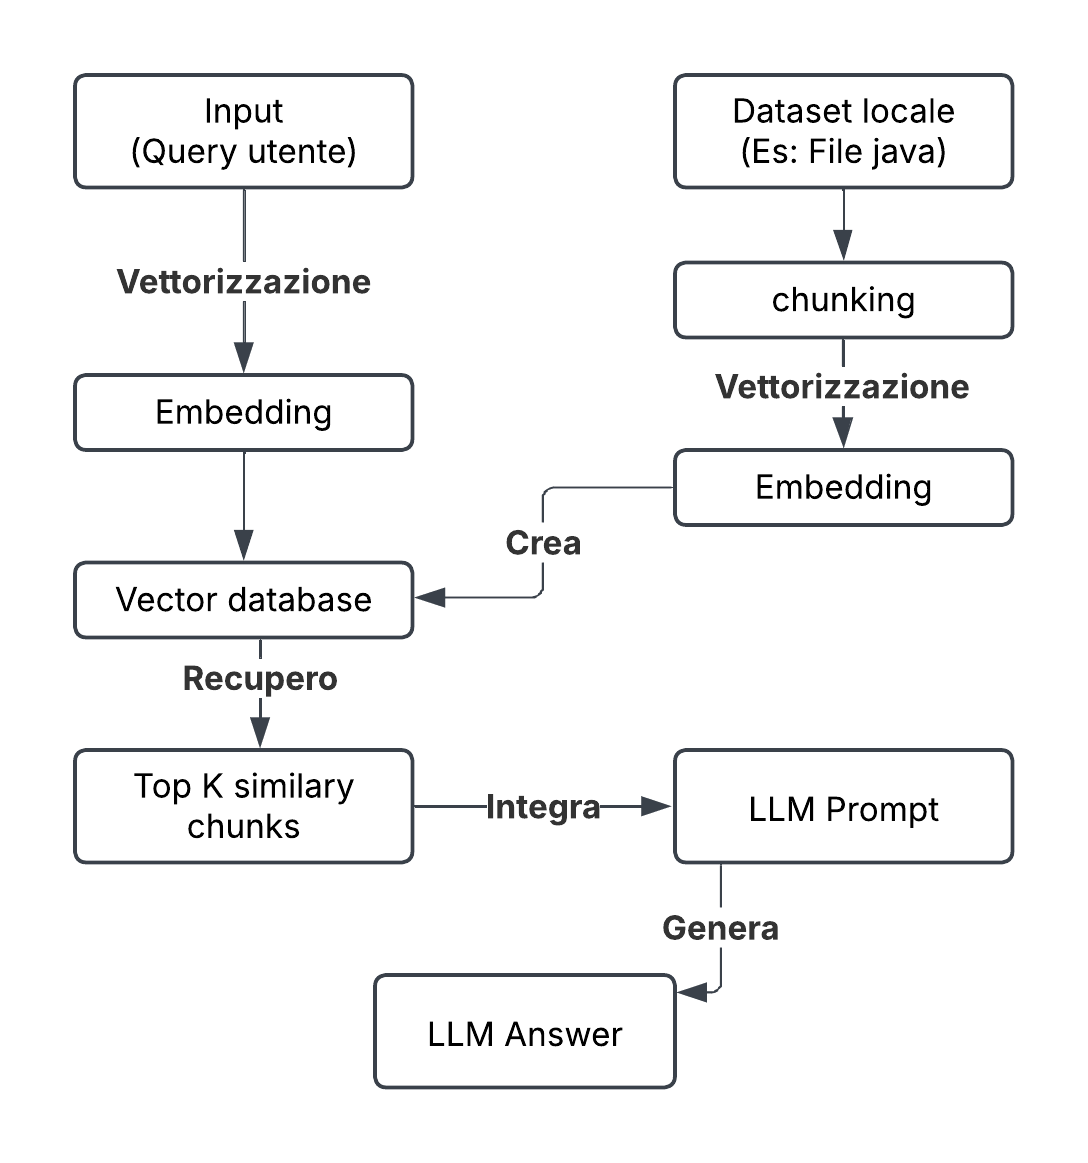
\includegraphics[width=0.8\linewidth]{figures/SistemaRAG.png}
    \caption{Funzionamento del sistema RAG}
    \label{fig:SistemaRAG.png}
\end{figure}

\subsection{Creazione Vector Database}
La propria \emph{knowledge base} deve essere salvata in un database vettoriale, in modo da poter essere interrogata in maniera efficiente dal sistema RAG.
Per creare questo database vengono utilizzati dati esterni al training set originale del LLM, provenienti da diverse fonti come:
\begin{itemize}
    \item API e database interni
    \item Archivi documentali
    \item File di testo e codice
\end{itemize}
La creazione di un database ben strutturato e \underline{la fase più importante} di tutto il processo, dividere il codice in chunk correttamente etichettando ogni elemento con i corretti metadati è fondamentale per la sucessiva fase di interrogazione.
Il processo di creazione del Vector Database segue la seguente pipeline:
\begin{itemize}
    \item \textbf{Chunking}: Per garantire che i modelli di embedding possano lavorare efficacemente, è necessario suddividere il dataset in chunk di dimensioni controllate.
    Questi chunk devono essere abbastanza piccoli da mantenere la focalizzazione semantica, ma sufficientemente grandi da fornire un contesto utile.
    Tipicamente, i chunk variano tra 512 e 4096 token.
    \item \textbf{Embedding}: Conversione dei chunk in vettori numerici ad alta dimensionalità, utilizzando tecniche di embedding come Word2Vec, GloVe o BERT.
    Questi vettori rappresentano il contenuto semantico dei chunk, consentendo al sistema di confrontare e recuperare le informazioni in base alla similarità tra i vettori.
    \item \textbf{Vector Store}: Memorizzazione degli embedding in un database vettoriale per consentire una rapida interrogazione e recupero delle informazioni.
    Questo database deve essere progettato per garantire un'efficienza computazionale ottimale, in modo da ridurre i tempi di risposta del sistema.
\end{itemize}
%Creazione degli Embedding


\subsection{Fase 1: User query e function calling}
Data la query d'input da parte dell'utente, il sistema RAG è avviato da una chiamata di funzione per ricercare nel
\textbf{Vector Database} i chunk più rilevanti per la query.
Nei modelli più complessi in RAG è di fatto un agente integrato nel sistema che viene chiamato all'occorrenza quando la base di conoscenza del LLM non è sufficiente per fornire una risposta adeguata,
in questo modo viene anche razionalizzato e ottimizzato il costo computazionale del processo,
attivato solo quando strettamente necessario.
Rimane comunque questo passaggio una scelta configurabile in base allo specifico utilizzo del sistema,
ad esempio per un azienda che utilizza il LLM solo per compiti specifici e sempre contestualizzati può essere configurato il sistema in modo che chiami
la funzione RAG sempre.
\subsection{Fase 2: Recupero delle Informazioni}
Quando l'utente sottopone una query:
\begin{itemize}
    \item La domanda viene convertita in un vettore ad alta dimensionalità
    \item Il sistema cerca nel database vettoriale i chunk più simili alla query, calcolando la distanza tra i vettori utilizzando tecniche di confronto come la similarità coseno o la distanza euclidea.
    In \cref{fig:Esempio distanze chunk e query} è rappresentata, riducendo a due dimensioni lo spazio vettoriale, la distanza devi vettori più simili trovati nel database e la query.
    \item Se trovate corrispondenze con un determinato \emph{score\_threshold}, i chunk vengono recuperati.
\end{itemize}

\begin{figure}[h]
    \centering
    \includegraphics[width=0.8\linewidth]{figures/plotSearch.png}
    \caption{Esempio di distanze tra chunk e query}  
    \label{fig:Esempio distanze chunk e query}
\end{figure}

\subsubsection{Calcolo dello \emph{score\_threshold}}
In questo contesto, il parametro \texttt{score\_threshold} \cite{langchain-retriever-score-threshold} viene utilizzato per filtrare i chunk restituiti in base alla loro somiglianza con la query.
La somiglianza viene tipicamente calcolata mediante la \emph{cosine similarity} tra le embedding della query e quelle dei documenti presenti nel database.
Ogni chunk viene associato a un punteggio che rappresenta il grado di somiglianza con la query, e solo i chunk con un determinato \texttt{score\_threshold} vengono restituiti.
Per leggere questo parametro va prestata particolare attenzione al tipo di somiglianza calcolata,
nella \emph{cosine similarity} il valore va da 0 è 1.
\subsection{Fase 3: Aumento del Prompt}
Il sistema \ac{RAG} arricchisce il Prompt dell'utente con le informazioni recuperate, fornendo al \ac{LLM} un contesto più ampio e dettagliato per generare una risposta coerente. In questo modo, il \ac{LLM} riceve un input contenente le informazioni relative alla risposta che dovrà generare. Unendo la sua base di conoscenza a queste informazioni esterne, riesce a rispondere in maniera molto più accurata e contestualizzata. Un Prompt aumentato con l'inserimento di Chunk è formato dai seguenti elementi:
\begin{itemize}
    \item \textbf{Query Utente}: 'Scrivi una funzione in Java che valuti la precisione dei tiri a Basket'
    \item \textbf{Chunk Recuperato}: 'chunk contenente una funzione che calcola la precisione dei tiri a Basket'
\end{itemize}
Inserendo all'interno del Prompt i chunk contenenti le informazioni necessarie per generare la risposta, è possibile guidare il LLM verso la soluzione. In questo modo si evita che il LLM parta da zero per arrivare alla risposta, ma parta già da una base che gli permette di generare una risposta più precisa e coerente.

\subsubsection{Aggiunta di informazioni di sistema}
In aggiunta ai chunk recuperati, è possibile inserire nel prompt delle informazioni di sistema, finalizzate a indirizzare le risposte del \ac{LLM}. Queste informazioni diventano parte integrante del flusso standard del RAG e sono sempre uguali, non dipendendo dalla query inserita, e hanno lo scopo di fornire al modello ulteriori dettagli, migliorando e personalizzando la qualità dell'output. Un esempio potrebbe essere la richiesta al \ac{LLM} di rispondere sempre utilizzando la valuta Dollaro. Scrivendo le query in italiano, il \ac{LLM} avrebbe proposto come valuta l'Euro, essendo la moneta utilizzata in Italia; ma con l'aggiunta di questa informazione, il modello risponderà sempre utilizzando come valuta il Dollaro.
\section{Perchè RAG}
Il più grande vantaggio dato dalla creazione di un sistema RAG è la possibilità di personalizzare le risposte del \ac{LLM} senza dover intervenire direttamente sulla sua conoscenza.
Questo permette di eseguire rapidamente aggiornamenti al Vector database del \ac{RAG}, in modo da mantenere sempre aggiornata la base di conoscenza del modello.

Numerose applicazioni moderne dimostrano l'efficacia di questo approccio:
\begin{itemize}
    \item I \textbf{GPTs} personalizzati di ChatGPT, che integrano documenti specifici per creare assistenti specializzati
    \item \textbf{Bing Chat} utilizza l'integrazione di risultati di ricerca in tempo reale per fornire risposte aggiornate e contestualizzate.
    \item \textbf{Framework come LangChain} permettono agli sviluppatori di costruire applicazioni basate su RAG, combinando LLM e sistemi di recupero delle informazioni per creare soluzioni personalizzate.
\end{itemize}
Le performance di un LLM addestrato su misura per le proprie esigenze sono migliori dei risultati ottenuti da un sistema RAG ma per quasi
tutte le aziende questo è impossibile perchè richiede costi difficilmente sostenibili ed è per questo che i RAG sono un ottimo compromesso tra costi e benefici.
Il \ac{RAG} non modifica il LLM ma lo integra, permettendo di ottenere risposte personalizzate e contestualizzate senza dover intervenire direttamente sul modello.
Riassumendo i vantaggi principali di un sistema RAG sono:
\begin{itemize}
    \item permette di ottenere risposte mirate e personalizzate contenti knowledge relativa a librerie e codice custom senza dover intervenire direttamente sul \ac{LLM}
    \item possibiltà di aggiornare rapidamente il Database con la base di conoscenza interna
    \item facilita l'assistenza da parte del modello nella fase di debugging migliorando la sua comprensione di sistemi complessi
    \item supporta la creazione di documentazione aggiornata
    \item permette all'interno di un Team di migliorare la coerenza del codice scritto da diversi programmatori proponendo librerie e standard comuni
\end{itemize}
\chapter{Implementazione di un sistema RAG per lo sviluppo di codice per il linguaggio Java}
\section{Obiettivo}
Questo caso studio si propone l'obiettivo di verificare il livello di personalizzazione e qualità delle risposte di un \ac{LLM} integrato con un sistema \ac{RAG} specializzato per lo sviluppo di codice Java.
Potenziando la query nel Prompt di input del LLM attraverso la creazione di un sistema RAG di supporto,
verranno costruite e analizzate singolarmente tutte le fasi che compongono il processo.
Il sistema RAG è stato testato con della classi JAVA custom create appositamente per il caso studio.
\subsubsection{Problema da affrontare:}
Chiamate a più livelli di classi e metodi, dove il RAG potrebbe non essere in grado di estrapolare
le informazione necessarie da inserire nel Prompt per ottenere dal LLM risposte coerenti con quanto richiesto.
\section{Architettura del Sistema}
\begin{figure}[H]
    \centering
    \begin{tikzpicture}[node distance=2cm]
        % Components
        \node [block] (chunk) {Text Processor\\(Chunking)};
        \node [block, right=of chunk] (embed) {Embedder\\(BGE-M3)};
        \node [block, right=of embed] (db) {Vector DB\\(FAISS)};
        \node [block, below=of chunk] (retriever) {Retriever};
        \node [block, right=of retriever] (llm) {LLM Interface\\(Es:CodeQwen)};
        
        % Connections
        \path [line] (chunk) -- (embed);
        \path [line] (embed) -- (db);
        \path [line] (db) -- (retriever);
        \path [line] (retriever) -- (llm);
        
        % Box around everything
        \node [draw, dashed, fit=(chunk) (embed) (db) (retriever) (llm),
            inner sep=1cm] {};
    \end{tikzpicture}
    \caption{Architettura del sistema RAG}
    \label{fig:rag-architecture}
\end{figure}
Il sistema RAG è stato progettato con un'architettura modulare che si compone di cinque componenti principali,
ognuna delle quali svolge un ruolo fondamentale nel trasformare dati grezzi in risposte coerenti e contestualizzate.
\subsection{Text Processor (Chunking)}
Il primo modulo, il \textbf{Text Processor (Chunking)}, si occupa di suddividere i file Java in chunk costituiti da un numero definito di token. Questa operazione non si limita a dividere il testo in parti uguali, ma è studiata per mantenere intatto il contesto del codice. Infatti, il sistema gestisce con attenzione la sovrapposizione dei token tra i chunk adiacenti, assicurandosi che nessuna informazione rilevante venga persa durante il processo di frammentazione.
\subsection{Embedder (BGE-M3)}
La fase successiva coinvolge l'\textbf{Embedder} basato sul modello BGE-M3. Questo componente trasforma i frammenti testuali in rappresentazioni vettoriali dense attraverso un processo di embedding multivettoriale.
Questi vettori vengono poi normalizzati, una procedura essenziale per ottimizzare le future ricerche di similarità nel database vettoriale.
\subsection{Vector DB (FAISS)}
L'archiviazione e la ricerca efficiente sono delegate al \textbf{Vector DB FAISS} (Facebook AI Similarity Search). 
Questo modulo memorizza gli embedding generati, organizzandoli in un database vettoriale che permette di eseguire ricerche basate sulla similarità. Grazie a questa struttura, il sistema può recuperare in modo rapido ed efficiente i chunk più rilevanti in risposta a specifiche query, garantendo prestazioni elevate anche in presenza di grandi quantità di dati.
\subsection{Retriever}
A completare il flusso operativo, il modulo \textbf{Retriever} esegue query semantiche sul database vettoriale. Analizzando i vettori e individuando quelli che meglio rispondono ai criteri di rilevanza, il Retriever estrae i k chunk più pertinenti e li organizza per creare un contesto ricco e strutturato. Questo contesto viene poi fornito al modello di linguaggio per permettergli di generare risposte il più possibile accurate e specifiche.
\subsection{LLM Interface}
Infine, l'\textbf{LLM Interface (CodeQwen e Llama 3.2)} rappresenta il punto di interazione diretto con l'utente. Attraverso un'interfaccia gestita da Ollama, questo modulo comunica con i modelli di linguaggio CodeQwen e Llama 3.2, utilizzando il contesto prelevato dal Retriever per generare risposte personalizzate e contestualizzate. In questo modo, il sistema RAG integra e potenzia le capacità del LLM senza modificare direttamente la sua base di conoscenza.
Nel complesso, l'architettura modulare del sistema RAG permette di combinare la flessibilità della generazione basata su LLM con la precisione e la rapidità dei sistemi di recupero delle informazioni, offrendo così una soluzione altamente efficace per la personalizzazione e l'aggiornamento continuo delle risposte generate.
\section{Software Utilizzati}
\subsection{Ollama\hspace{0.3cm}\protect\includegraphics[width=0.03\linewidth]{figures/ollama.png}}
Ollama \cite{ollama-docs} è un software che permette di utilizzare in locale LLM
senza dover dipendere da servizi cloud esterni.
Il software è stato scelto per la sua flessibilità, permettendo di integrare facilmente i modelli LLM nel sistema RAG.

\subsection{Llama 3.2}
Llama 3.2 3B \cite{llama3-2}, un language model open source.
Il modello, con 3 miliardi di parametri, è ottimizzato per compiti di dialogo multilingue e si distingue per le sue capacità di recupero e sintesi delle informazioni.
La scelta è ricaduta su questa versione per il suo equilibrio tra prestazioni e requisiti computazionali che permottono il suo utilizzo senza hardware troppo potente.

\subsection{Codeqwen 1.5}
Codeqwen \cite{codeqwen1.5} è un language model open source specializzato nella generazione di codice e documentazione tecnica.  
Con 7 miliardi di parametri, il modello è stato addestrato su un ampio dataset di codice sorgente e documentazione tecnica, permettendo di generare codice coerente e ben strutturato.
La scelta di questo modello è stata dettata, a differenza di llama3.2, dalla sua specializzazione nella programmazione e dalla sua capacità di generare codice di alta qualità. 
%\subsubsection{qwen2.5-coder:3b}
%qwen2.5-coder \cite{qwen-coder} è stato sviluppato da Qwen AI ed è anchesso open source, specializzato nella generazione di codice e documentazione tecnica.
%Con 3 miliardi di parametri, il modello è stato addestrato su un ampio dataset di codice sorgente e documentazione tecnica, permettendo di generare codice coerente e ben strutturato. 
%La scelta di questo modello è stata dettata, a differenza di llama3.2, dalla sua specializzazione nella programmazione e dalla sua capacità di generare codice di alta qualità.

\subsection{LangChain}
LangChain \cite{langchain} è un framework open source progettato per costruire applicazioni basate su LLM.
Fornisce strumenti avanzati per integrare modelli con dati esterni ed API, creare pipeline con chain
e gestire database vettoriali, supportando l'implementazione di sistemi RAG.

\subsection{BGE-M3}
BGE-M3 \cite{bge-m3} è un modello di embedding testuale open source per la gestione di dati strutturati e non strutturati multilingue.
Il modello permettendo di convertire testo in vettori numerici ad alta dimensionalità.

\subsection{FAISS}
FAISS (Facebook AI Similarity Search) \cite{faiss} è una libreria open source per la ricerca efficiente di similarità e il clustering di vettori densi.
Progettata per gestire dataset su larga scala, FAISS supporta operazioni di ricerca anche su insiemi di vettori che superano la capacità della RAM, grazie a tecniche di indicizzazione avanzate e ottimizzazioni computazionali.
\section{Dataset}
Il dataset è stato creato appositamente per testare il sistema RAG ed è composto da diciannove classi Java.
\'E possibile scaricare il dataset in \url{https://github.com/ilBollo/Tesi/tree/main/my_project/classi_java_custom}
Il dataset è composto dalle seguenti classi Java: 
\begin{description}
    \item[DateUtilCustom.java] Classe personalizzata per gestire le date
    \item[GiorniMagici.java] Classe per calcolare in maniera particolare dei giorni
    \item[BasketballStats.java] Classe abstract per statistiche di basket
    \item[AdvancedBasketballStats] Classe che estende BasketballStats
    \item[BasketballTest] Classe per testare le statistiche di basket implementate in AdvancedBasketballStats
    \item[Altre classi java] Non strettamente correlate con le prime due utili per aumentare la base dati sul quale effettuare le ricerche e per testare la capacità di generalizzazione del sistema.
\end{description}
\section{Risultato atteso caso d'uso RAG}
DateUtilCustom.java e GiorniMagici.java sono strettamente correlate infatti GiorniMagici.java richiama metodi definiti in DateUtilCustom.java.
Inizialmente andremo a testare il sistema RAG impostando come primo input la seguente query: 
\begin{itemize}
    \item \textbf{Cosa ritorna il metodo \texttt{segnaleWow(LocalDate.of(2025, 2, 14))}?}
\end{itemize}

\subsection{Codice di riferimento per rispondere alla query}
In GiorniMagici.java è presente la seguente funzione:
\begin{lstlisting}[language=Java, caption={Metodo segnaleWow in GiorniMagici.java}, label={lst:segnaleWow}]
public static String segnaleWow(LocalDate data) {
    String wow = "il tuo segnale Wow e': " + DateUtilCustom.getMessaggioMagico(data);
    return wow;
}
\end{lstlisting}
Questa funzione richiama il metodo \texttt{getMessaggioMagico} presente in DateUtilCustom.java:

\begin{lstlisting}[language=Java, caption={Metodo getMessaggioMagico in DateUtilCustom.java}, label={lst:getMessaggioMagico}]
public static String getMessaggioMagico(LocalDate datamagica) throws DateTimeParseException {
    DayOfWeek giornoSettimana = datamagica.getDayOfWeek();
    switch(giornoSettimana) {
        case MONDAY: return "La magia inizia nel silenzio...";
        case TUESDAY: return "I sussurri degli antichi si fanno sentire.";
        case WEDNESDAY: return "Il velo tra i mondi e' sottile oggi.";
        case THURSDAY: return "L'energia magica e' potente e chiara.";
        case FRIDAY: return "Attenzione agli incantesimi del crepuscolo.";
        case SATURDAY: return "Il giorno perfetto per scoprire segreti nascosti.";
        case SUNDAY: return "Riposa e rigenera il tuo potere magico.";
        default: return "Il giorno e' avvolto nel mistero...";
    }
}
\end{lstlisting}

\subsection{Output}
Il sistema RAG dovrebbe essere in grado di recuperare i chunk relativi ai metodi \texttt{segnaleWow} e \texttt{getMessaggioMagico} e di integrarli nel Prompt del LLM.
Il modello, basandosi su queste informazioni, dovrebbe generare una risposta coerente e contestualizzata alla query iniziale.
Nel caso specifico essendo il 14 Febbraio 2025 un venerdì,  la risposta corretta è:
\begin{quote}
    \textbf{``il tuo segnale Wow è: Attenzione agli incantesimi del crepuscolo.''}
\end{quote}
\section{Implementazione}
\subsection{Chunking del Codice Java}
Per segmentare il codice Java in chunk, è stata utilizzata la libreria \texttt{langchain\_text\_splitters}.
Durante la progettazione del sistema di chunking, sono state analizzate le caratteristiche del codice Java e sono state adottate specifiche strategie per garantire una suddivisione efficace e accurata:
\begin{itemize}
    \item La dimensione dei chunk è stata impostata a 512 token. 
    Questa scelta è stata fatta per evitare che metodi diversi vengano fusi nello stesso chunk, garantendo al contempo un contesto sufficientemente utile.
    \item È stato introdotto un overlap di 128 token tra i chunk. Questo assicura una continuità tra i chunk adiacenti, evitando la perdita di informazioni rilevanti.
    \item Sono stati utilizzati separatori specifici per il linguaggio Java, come \texttt{\textbackslash n\}\textbackslash n\textbackslash npublic}, \texttt{\textbackslash nclass}, e \texttt{\textbackslash n/***}.
    Questi separatori aiutano a preservare la struttura logica del codice.
    \item Sono state implementate espressioni regolari per estrarre i nomi dei metodi e delle classi dai chunk.
    Queste espressioni permettono di identificare i metodi e le classi presenti nel codice, arricchendo i chunk con informazioni contestuali.
\end{itemize}
\newpage
\subsubsection{Funzione process\_file\_Java parte 1: Inizializzazione e Configurazione}
\begin{lstlisting}[language=Python, caption={Configurazione dello splitter}]
    def process_file_Java(file_path):
        with open(file_path, "r", encoding="utf-8") as f:
            lines = f.readlines()
        text = ''.join(lines)
        splitter = RecursiveCharacterTextSplitter(
            chunk_size=512,
            chunk_overlap=128,
            separators=[    # Separatori basati sulla sintassi Java
                "\n}\n\npublic ",
                "\n}\n\nprivate ",
                "\n}\n\nprotected ",
                "\n}\n\nstatic ",
                "\n}\n\n// End of method", 
                "\nclass ",  # Inizio nuove classi
                "\n@",      # Annotazioni
                "\n/**",    # Javadoc
                "\n * ", 
                "\n"
            ],
            keep_separator=True, # Mantiene i separatori nei chunk
            is_separator_regex=False # Separatori letterali (non regex)
        )
\end{lstlisting}
Nella prima parte la funzione:
\begin{itemize}
    \item Legge il file Java e unisce il contenuto in un unico blocco di testo
    \item Configura \texttt{RecursiveCharacterTextSplitter} con:
    \begin{itemize}
        \item Separatori specifici per costrutti Java (metodi, classi, annotazioni)
        \item Token di dimensione 512 e overlap di 128
        \item Mantenimento dei separatori nei chunk e uso di separatori letterali
    \end{itemize}
\end{itemize}

\subsubsection{Funzione process\_file\_Java parte 2: Generazione dei Chunk e Metadati}
\begin{lstlisting}[language=Python, caption={Generazione chunk e metadati}]
    # Suddivisione del testo e calcolo metadati
    chunks = splitter.split_text(text)
    chunk_metadata = []
    cursor = 0
    
    for chunk in chunks:
        # Calcolo righe di inizio/fine
        start_line = text.count('\n', 0, cursor) + 1
        chunk_length = len(chunk)
        end_line = text.count('\n', 0, cursor + chunk_length) + 1
        
        # Estrazione contesto semantico
        method_name = extract_method_name(chunk)
        
        # Registrazione metadati
        chunk_metadata.append({
            "start_line": start_line,
            "end_line": end_line,
            "text": chunk,
            "methods": [method_name]
        })
        cursor += chunk_length
    
    return chunk_metadata
\end{lstlisting}

Nella seconda parte la funzione:
\begin{itemize}
    \item Calcola le righe di inizio/fine con logica a cursore
    \item Arricchisce ogni chunk con i metadati sfruttando anche la funzione \texttt{extract\_method\_name} per estrarre i nomi dei metodi
    \item Ritorna una lista di chunk con i relativi metadati
\end{itemize}


\subsubsection{Funzione extract\_method\_name}
Per arricchire ulteriormente i chunk è stata creata la funzione \texttt{extract\_method\_name}.
Questa funzione identifica i nomi dei metodi e delle classi all'interno dei chunk utilizzando espressioni regolari (regex).
 n questo modo, ogni chunk può essere associato a un contesto semantico specifico, migliorando la ricerca in fase di embedding e arricchendo il Prompt del LLM con informazioni contestuali.

\begin{lstlisting}[language=Python, caption={Estrazione contesto dai chunk}]
    def extract_method_name(text):
    # Pattern per la firma di un metodo in Java
    method_pattern = r'(?:public|private|protected|static|final|synchronized|abstract|native)\s+[\w<>\[\]]+\s+(\w+)\s*\([^)]*\)'
    # Pattern per i costruttori
    constructor_pattern = r'(?:public|private|protected)\s+(\w+)\s*\([^)]*\)'
    
    # Cerca la firma di un metodo
    matches = re.findall(method_pattern, text)
    if matches:
        return matches[0]  # Restituisce il primo metodo trovato
    
    # Cerca costruttori
    constr_matches = re.findall(constructor_pattern, text)
    if constr_matches:
        return constr_matches[0] + " (costruttore)"
    
    # Cerca chiamate a metodi
    method_calls = re.findall(r'\.(\w+)\s*\(', text)
    if method_calls:
        return f"Chiamata a: {method_calls[-1]}"
    return "unknown_method"
\end{lstlisting}

\subsubsection{Metadato Class}
Durante l'elaborazione dei file, è importante mantenere traccia del contesto delle classi.
Questo viene fatto aggiornando dinamicamente il nome della classe corrente mentre si processano i chunk.
In questo modo, ogni chunk può essere associato alla classe corretta.

\begin{lstlisting}[language=Python, caption={Aggiornamento contesto classe}]
current_class = ""
for file_path in files:
    chunks_info = process_file_Java(file_path)
    for chunk_info in chunks_info:
        if "class " in chunk_info["text"]:
            class_name = chunk_text.split("class ")[1].split("{")[0].strip()
            current_class = class_name
        all_chunks.append({..., "class": current_class})
\end{lstlisting}

\subsubsection{Creazione file json}
Il risultato finale del processo di chunking viene salvato in un file json chiamato \texttt{chunks.json}.
Questo file contiene la lista dei chunk, ognuno dei quali comprende i metadati come il percorso del file originale, la relativa classe, i metodi identificati e le linee di codice di inizio e fine.
\'E stato inserito di default il campo \texttt{type} per identificare il tipo di chunk, in questo caso \texttt{code}.
Questo dato apre la possibilità di estendere il sistema per supportare altri tipi di chunk, come testo libero o documentazione.
\begin{lstlisting}[language=json, caption={Esempio di chunk generato}]
[
    {
        "id": 1,
        "text": "package classi_java_custom;\nimport java.time.LocalDate;...",
        "source": "my_project/.../AdvancedBasketballStats.java",
        "type": "code",
        "start_line": 1,
        "end_line": 14,
        "class": "AdvancedBasketballStats extends BasketballStats",
        "methods": ["calcolaEfficienzaGiocatore"]
    }
]
\end{lstlisting}
\subsection{Generazione degli Embedding}
Gli embedding trasformano i chunk in rappresentazioni vettoriali che catturano il significato semantico.
Il seguente codice Python mostra come generare gli embedding e creare un database Faiss.
Come precedentemente descritto, il modello di embedding utilizzato è BGE-M3, questo modello usa due rappresentazioni per complementarietà, la rappresentazione densa cattura relazioni semantiche mentre quella sparsa cattura relazioni sintattiche.
Mentre sul database FAISS ad alta dimensionalità verrà settata la ricerca di somiglianza utilizzando la distanza euclidea tra i vettori.
    \begin{lstlisting}[language=Python, caption={Generazione degli embedding e creazione di un database FAISS}, label={lst:embeddings}]
        from sentence_transformers import SentenceTransformer
        from langchain_community.vectorstores import FAISS
        
        # 1. Carica i chunk dal file JSON
        with open("chunks.json", "r", encoding="utf-8") as f:
            chunks_data = json.load(f)        
        chunks = [item["text"] for item in chunks_data]
        
        # 2. Carica il modello BGE-M3 e genera gli embedding
        embedder = SentenceTransformer('BAAI/bge-m3')
        embeddings = embedder.encode(
            [
                f"METHODS:{', '.join(c['methods']) if c['methods'] else 'unknown'}" 
                f"CLASS:{c['class']}"
                f"LINES:{c['start_line']}-{c['end_line']}"
                f"CONTENT:{c['text']}"
                for c in chunks_data
            ],
            show_progress_bar=True
        )
        
        # 3. Crea un database FAISS
        vector_store = FAISS.from_embeddings(
            text_embeddings=list(zip(chunks, embeddings)),  # Abbina testi e embedding
            embedding=embedder,  # Modello per future operazioni
        )
        
        # 4. Salva il database
        vector_store.save_local("./faiss_db")
        print("Database FAISS creato e salvato in ./faiss_db.")
    \end{lstlisting}
Il metodo \emph{encode} del modello BGE-M3 genera gli embedding per ogni chunk,
arricchendoli con i metadati creati durante il processo di chunking.
Questi embedding vengono poi utilizzati per creare un database FAISS, che permette di eseguire ricerche di similarità in modo efficiente.
\subsection{Esecuzione di query sul Database FAISS}
    Una volta creato il database FAISS, è possibile eseguire ricerche semantiche sui chunk memorizzati:

    \begin{lstlisting}[language=Python, caption={Esecuzione di una query sul database FAISS}, label={lst:query}]
    # 1. Carica il modello di embedding nel formato corretto
    embedder = HuggingFaceEmbeddings(
        model_name="BAAI/bge-m3",
        model_kwargs={'device': 'cpu'},
        encode_kwargs={'normalize_embeddings': True}
    )

    # 2. Carica il database FAISS esistente
    vector_store = FAISS.load_local(
        folder_path="./faiss_db",
        embeddings=embedder,
        allow_dangerous_deserialization=True
    )

    # 3. Query di esempio
    query = "Cosa ritorna il metodo segnaleWow(LocalDate.of(2025, 1, 10))?"

    # 4. Cerca i chunk piu' simili
    docs = vector_store.similarity_search_with_score(
        query,
        k=5,
        score_threshold=0.90,  # bassa similarita'
        search_type="similarity",  # Piu' efficace per il codice
        lambda_mult=0.5       # Bilancia diversita'/rilevanza
    )
    # 5. Stampa i risultati con relativo score
    for i, (doc, score) in enumerate(docs):
        print(f"Risultato {i+1} (Score: {score:.4f}):")
        print(doc.page_content)
        print("-" * 40)
    \end{lstlisting}
LangChain fornisce un'interfaccia semplice per eseguire query semantiche sul database FAISS.
\subsubsection{Parametri di ricerca}
\begin{itemize}
    \item \textbf{k}: Questo parametro definisce il numero di chunk da restituire in risposta a una query. In questo caso, \texttt{k=5} restituisce, se trovati, i 5 chunk più rilevanti.
    \item \textbf{score\_threshold}: Questo parametro definisce il valore minimo di similarità richiesto per considerare un chunk come rilevante. Il parametro \texttt{score\_threshold} ripartisce i valori con una scala inversa rispetto alla cosine similarity. In questo esempio, filtrando chunk con un valore minore o uguale a 0.90 si ottengono chunk con un grado di somiglianza medio-bassa.
    \item \textbf{search\_type}: Questo parametro definisce il tipo di ricerca da eseguire sul database FAISS. La scelta \texttt{search\_type="similarity"} (similarità del coseno) è efficace per il codice per tre motivi chiave:
    \begin{itemize}
        \item \textbf{Cerca somiglianze nella logica}, non nella forma: Ignora differenze come:
        \begin{itemize}
            \item Nomi variabili diversi (es. \texttt{data} vs \texttt{date})
            \item Commenti o spaziature extra
            \item Lunghezza del codice
        \end{itemize}
        \item \textbf{Trova funzioni equivalenti}: Riconosce che due metodi sono simili anche se:
        \begin{itemize}
            \item Usano librerie diverse ma fanno la stessa cosa
            \item Hanno parametri leggermente diversi
            \item Sono scritti in stili differenti
        \end{itemize}
        \item \textbf{Migliora la ricerca semantica}: Capisce che:
        \begin{itemize}
            \item \texttt{calcolaMedia()} e \texttt{getAverage()} possono essere equivalenti
            \item Un costruttore e un metodo factory sono correlati
            \item Un loop \texttt{for} e un loop \texttt{while} implementano la stessa logica
        \end{itemize}
    \end{itemize}
\end{itemize}

    \subsubsection{Chunk estratti con query base}
    Testiamo il risultato con una query sintetica, senza alcun riferimento esplicito al metodo utilizzato all'interno di segnale Wow.
    \begin{itemize}
        \item \textbf{Query:} 
            `Cosa ritorna il metodo segnaleWow(LocalDate.of(2025, 1, 10))?'
        \item \textbf{Output:}
        viene restituito il chunk corretto con uno score di similarità di \textbf{0.6457}. Questo valore non è particolarmente basso ma sufficiente per identificare il chunk corretto.
    \end{itemize}
    \paragraph{Nota:}
    È importante riscontrare che viene restituito un solo chunk nonostante \texttt{k=5}.
    Questo accade perché nessun altro chunk supera la soglia di similarità impostata.
    Tale comportamento evidenzia una criticità: la funzione \texttt{segnaleWow()} richiama un metodo presente nella libreria \texttt{DateUtilCustom} che non viene estratto dal Dataset.

    \subsubsection{Query che descrive il contesto in maniera più completa}
    Alla query iniziale vien aggiunto il riferimento al metodo utilizzato all'interno di segnale Wow.
        \begin{itemize}
            \item \textbf{Query:}
                `Cosa ritorna il metodo segnaleWow(LocalDate.of(2025, 1, 10)) che utilizza la funzione getMessaggioMagico() della libreria DateUtilCustom?'
            \item \textbf{Output:}
            Fornisce i seguenti cinque chunk.
            \begin{itemize}
                \item Primo chunk \textbf{(score: 0.5082)}: contiene la funzione \texttt{segnaleWow}
                \item Secondo, terzo e quarto chunk \textbf{(scores: 0.7132, 0.7611, 0.8084)}: contengono la funzione \texttt{getMessaggioMagico}
                \item Quinto chunk \textbf{(score: 0.8239)}: funzione non rilevante relativa alle date
            \end{itemize}
        \end{itemize}

    \subsubsection{Conclusione}
    Sono stati riscontrati due problemi molto rilevanti, il primo riguarda la mancanza di estrazione di metodi da librerie esterne se non esplicitate nella query.
    Mentre il secondo è causato da i chunk estratti, lo score impostato non è particolarmente basso e questo può causare l'estrazione di chunck relativi a funzioni con terminologie e meccanismi simili ma non coerenti con il contesto cercato.
    Per questo secondo punto questa analisi ha portato alla decisione di abbassare \texttt{score\_threshold} da 0.90 a 0.82,
    questa piccola correzione risolve in parte il problema o almeno evita di propagarlo ulteriormente, preferendo non ottenere in certi casi risultati dal \ac{RAG} piuttosto che ricevere risposte non coerenti.
\subsection{Creazione della Pipeline RAG}
La pipeline RAG combina i componenti precedentemente descritti per creare un sistema completo di generazione di risposte.
\begin{lstlisting}[language=Python, caption={Caricamento database FAISS}, label={lst:Caricamento database FAISS}]
    # Configurazione embedding
    embedder = HuggingFaceEmbeddings(
        model_name="BAAI/bge-m3",
        model_kwargs={'device': 'cpu'},
        encode_kwargs={'normalize_embeddings': True}
    )
    # Caricamento database FAISS
    vector_store = FAISS.load_local(
        folder_path="./faiss_db",
        embeddings=embedder,
        allow_dangerous_deserialization=True
    )
\end{lstlisting}
Inizialmente per eseguire l'embedder della query di input viene utilizzato il modello BAAI/bge-m3 e caricato il database FAISS precedentemente creato.

\begin{lstlisting}[language=Python, caption={Configurazione Parametri}, label={lst:Configurazione Parametri}]
    # Creazione del retriever
    retriever=vector_store.as_retriever(
        search_kwargs={
            "k": 5,                   # Piu' documenti per contesto
            "score_threshold": 0.82, # medio-bassa similarita' inizialmente era 0.90
            "search_type" :"similarity",  # Piu' efficace per il codice
            "lambda_mult":0.5       # Bilancia diversita'/rilevanza
        }
    )
    # Comando di sistema
    varStileLLM = "Sei un assistente che combina codice Java e contesto strutturale per risposte precise."

    # Configurazione Template del prompt specifici per i modelli
    LLAMA_TEMPLATE = """<|begin_of_text|>
    <|start_header_id|>system""" + varStileLLM + """<|end_header_id|>
    Contesto: {context}<|eot_id|>
    <|start_header_id|>user<|end_header_id|>
    Domanda: {input}<|eot_id|>
    <|start_header_id|>assistant<|end_header_id|>"""

    CODEQWEN_TEMPLATE = """<|im_start|>system """ + varStileLLM + """
    {context}<|im_end|>
    {{ if .Functions }}<|im_start|>functions
    {{ .Functions }}<|im_end|>{{ end }}
    <|im_start|>user
    {input}<|im_end|>
    <|im_start|>assistant
    """

    COMMON_PARAMS = {
        "temperature": 0.3, #lasciamo una bassa creativita' non vogliamo che inventi risposte
        "top_p": 0.85  # Bilancia creativita'/controllo nei token generati
    }
\end{lstlisting}
Il retriever viene configurato con i parametri di ricerca precedentemente descritti.
Vengono inoltre definiti i template del prompt per i due modelli LLM, Llama3.2 e Codeqwen, con il parametro system = \texttt{varStileLLM} e il tag context dove verranno inseriti i chunk recuperati dal database FAISS.
I COMMON\_PARAMS sono stati impostati rispettivamente a:
\begin{itemize}
    \item \textbf{temperature}: 0.3, in modo da garantire risposte coerenti e precise senza inventarle.
    \item \textbf{top\_p}: 0.85, per bilanciare creatività e controllo nei token generati.
\end{itemize}
\subsubsection{varStileLLM}
Come parametro di sistema da passare al LLM è stata creata la variabile \texttt{varStileLLM} con il seguente valore: \textbf{``Sei un assistente che combina codice Java e contesto strutturale per risposte precise.''}
questo parametro sarà passato ad ogni Prompt generato per il LLM e condizionerà tutte le risposte fornite.

\begin{lstlisting}[language=Python, caption={Caricamento del modello}, label={lst:Caricamento del modello}]
    # Caricamento modello
def load_model(model_name):
    models = {
        "llama3.2": {
            "template": LLAMA_TEMPLATE,
            "params": COMMON_PARAMS
        },
        "codeqwen": {
            "template": CODEQWEN_TEMPLATE,
            "params": COMMON_PARAMS
        }
    }
    if model_name not in models:
        raise ValueError(f"Modello non supportato: {model_name}")
    return OllamaLLM(
        model=model_name,
        **models[model_name]["params"]
    ), PromptTemplate(
        template=models[model_name]["template"],
        input_variables=["input", "context"]
    )

# Inizializza il modello
llm, prompt = load_model("codeqwen")
\end{lstlisting}
\textbf{load\_model} carica il modello LLM e il template del Prompt in base al modello scelto sfruttando OllamaLLM e PromptTemplate.
\begin{lstlisting}[language=Python, caption={Catena RAG}, label={lst:Catena RAG}]
# Catena RAG
document_chain = create_stuff_documents_chain(llm, prompt)
rag_chain = create_retrieval_chain(
    retriever,
    document_chain
)

# Funzione query
def ask_ollama(question):
    try:
        result = rag_chain.invoke({"input": question})
        print("DOMANDA:", question)
        print("RISPOSTA:")
        print(result["answer"])
        print("FONTI:")
        for i, doc in enumerate(result["context"], 1):
            print(f"{i}. {doc.page_content[:150]}...")
            if 'source' in doc.metadata:
                print(f" Fonte: {doc.metadata['source']}")
            print("-" * 80)
    except Exception as e:
        print(f"ERRORE: {str(e)}")

# Esempio d'uso
if __name__ == "__main__":
    ask_ollama("Cosa ritorna il metodo segnaleWow(LocalDate.of(2025, 2, 14)) che utilizza la funzione getMessaggioMagico() della libreria DateUtilCustom?")
    #ask_ollama("Cosa ritorna il metodo segnaleWow(LocalDate.of(2025, 2, 14))?")

\end{lstlisting}
La chiamata iniziale alla funzione \emph{ask\_ollama} richiede come parametro la query di input per poi essere processata dalla pipeline RAG.
Sfruttando le funzionalità della libreria LangChain \cite{langchain-retrieval-chain}, \textbf{\emph{result}} è un array contente la risposta e il contesto fornito alla query.
\subsubsection{\emph{rag\_chain.invoke}}
 Questa funzione esegue la catena RAG creata tramite il metodo \emph{create\_retrieval\_chain} che prende come parametri il retriever e il document chain.
 \begin{itemize}
    \item la funzione \textbf{create\_stuff\_documents\_chain()} carica una catena di documenti prendendo in input il modello LLM e il template del prompt.
 \end{itemize}
\section{Test Sistema RAG}
Valutiamo se il sistema RAG  è in grado di rispondere in maniera coerente alla query proposta.
Ricordiamo che il risultato atteso è: \textbf{``il tuo segnale Wow è: Attenzione agli incantesimi del crepuscolo.''}
\subsubsection{Modifica Temperature}
I LLM provavano a dare risposta anche senza avere tutte le informazioni necessarie, ho deciso di abbassare la temperatura da 0.3 a 0.2 per vedere se i modelli rispondessero in maniera più precisa.
Il risultato è stato raggiunto.
\subsection{Query base senza riferimenti al metodo utilizzato all'interno di segnaleWow}
\begin{quote}
    \texttt{``Cosa ritorna il metodo segnaleWow(LocalDate.of(2025, 2, 14))?''}
\end{quote}
\subsubsection{Fonti aggiunte al Prompt}
Il RAG aggiunge solo il chunk dove è presente la funzione \texttt{segnaleWow} e non il chunk con la funzione \texttt{getMessaggioMagico} della libreria DateUtilCustom
per questo le risposte dei due modelli sono incomplete:
\subsubsection{Output con LLM Llama3.2}
L'output ottenuto utilizzando il modello Llama3.2 è stato:
\begin{quote}
    ``Il metodo `segnaleWow` prende un parameetro di tipo `LocalDate` e lo utilizza per richiamare la funzione `getMessaggioMagico` di `DateUtilCustom`. Tuttavia, non è chiaro che il metodo `getMessaggioMagico` restituisca sempre una stringa.
    Supponendo che `getMessaggioMagico` ritorni sempre una stringa, il risultato del metodo `segnaleWow` con l'input `LocalDate.of(2025, 2, 14)` sarebbe:
    "il tuo segnale Wow è :messaggio magico"
    Tuttavia, senza sapere cosa esattamente ritorni `getMessaggioMagico`, non possiamo essere certi del risultato.''
\end{quote}

\subsubsection{Output con LLM CodeQwen}
CodeQwen continua a cercare di dare risposta senza conoscerla anche con la temperatura a 0.2, è stata quindi ulteriormente abbassata a 0.1 e top\_p è stato abbassato a 0.6.
Il modello continuava a dare risposte incomplete è stato quindi aggiunto alla variabile \emph{varStileLLM} la stringa \texttt{``Rispondi solo se hai certezza sicura della risposta.''}.
La risposta senza allucinazioni è stata:
\begin{quote}
    ``Il metodo `segnaleWow` restituisce una stringa che contiene un messaggio di "il tuo segnale Wow è :" seguito da un messaggio magico generato dal metodo `getMessaggioMagico` della classe `DateUtilCustom`.
    Per ottenere il valore del messaggio magico associato a una data specifica, ad esempio `LocalDate.of(2025, 2, 14)`, dovresti richiamare il metodo `getMessaggioMagico` direttamente su quella data:
    ```java
    String wow = DateUtilCustom.getMessaggioMagico(LocalDate.of(2025, 2, 14));
    System.out.println(wow);
    ```''
\end{quote}

\subsection{Risultati con query che descrive accuratamente il contesto}
Rieseguiamo il test ma con una query più dettagliata aggiungento i riferimenti al metodo utilizzato all'interno della funzione segnaleWow:
\begin{quote}
    \texttt{``Cosa ritorna il metodo segnaleWow(LocalDate.of(2025, 2, 14)) che utilizza la funzione getMessaggioMagico() della libreria DateUtilCustom?''}
\end{quote}
\subsubsection{Fonti aggiunte dal RAG al Prompt}
In questo caso il RAG aggiunge 4 chunk, il primo che riporta la funzione \texttt{segnaleWow} e gli altri tre chunk sonoo relativi alla funzione \texttt{getMessaggioMagico} della libreria DateUtilCustom.
Ne consegue che \textbf{le risposte date dai due modelli sono coerenti con quanto atteso}.
\subsubsection{Output con LLM Llama3.2}
``Il metodo `segnaleWow` restituisce una stringa che contiene il messaggio magico per la data specificata. Tuttavia, il messaggio magico è generato dalla funzione `getMessaggioMagico` della libreria `DateUtilCustom`, che richiede un oggetto `LocalDate`.
Il problema è che il metodo `segnaleWow` non restituisce direttamente il messaggio magico, ma piuttosto una stringa che contiene il messaggio magico. Quindi, per ottenere il messaggio magico effettivamente, dobbiamo chiamare entrambi i metodi.
Ecco la soluzione:
```java
public static String segnaleWow(LocalDate date) {
    return "Il tuo segnale Wow è: " + getMessaggioMagico(date);
}
```
Quindi, se chiamiamo `segnaleWow` con una data specifica, otteniamo il messaggio magico come risultato:
```java
LocalDate date = LocalDate.of(2025, 2, 14);
String messaggioMagico = segnaleWow(date);
System.out.println(messaggioMagico); // "Il tuo segnale Wow è: Il giorno perfetto per scoprire segreti nascosti."
```
In questo modo, otteniamo il messaggio magico effettivamente.''

\subsubsection{Output con LLM CodeQwen}
``Il metodo `segnaleWow` restituisce una stringa che contiene il messaggio magico associato alla data specificata. In questo caso, se si utilizza la funzione `getMessaggioMagico(LocalDate.of(2025, 2, 14))`, la data è un lunedì (14 febbraio 2025).
Il metodo `getMessaggioMagico` restituisce il messaggio magico associato al giorno della settimana del parametro `datamagica`. Nel caso di una data lunedì, il messaggio restituito sarà "La magia inizia nel silenzio...".
Quindi, la risposta del metodo `segnaleWow(LocalDate.of(2025, 2, 14))` sarà:
```
il tuo segnale Wow è : La magia inizia nel silenzio...''
\subsection{Commento risultati ottenuti}
I risultati ottenuti mostrano come il sistema RAG sia in grado di rispondere in maniera coerente alla query proposta.
La ricerca dei chunk più simili funziona correttamente soprattutto se si scrive la richiesta in maniera più dettagliata possibile.
I LLM hanno sbagliato a calcolare il giorno della settimana a causa di un loro errore nel calcolare il giorno della settimana corrispondente alla data fornita come parametro.
Ma le risposte fornite utilizzano correttamente il metodo getMessaggioMagico.
Sono stati migliorati i parametri di ricerca per evitare allucinazioni da parte dei modelli.
Eseguendo questo test utilizzando versioni di questi modelli con più parametri, si è ottenuto il risultato corretto.
\subsubsection{Esempio utilzzando qwen con 70 bilioni di parametri}
Testato su https://deepinfra.com/Qwen/Qwen2.5-Coder-7B dove è stato possibile settare anche gli stessi parametri al modello, ovvero temperature 0.1 e top\_p 0.6.
\begin{quote}
    \texttt{`` Il metodo `segnaleWow(LocalDate.of(2025, 2, 14))` ritorna una stringa che contiene il messaggio magico corrispondente alla data fornita. In questo caso, la data è il 14 febbraio 2025, che è un venerdì. Quindi, il metodo `getMessaggioMagico(LocalDate datamagica)` restituirà il messaggio "Attenzione agli incantesimi del crepuscolo." 
    Quindi, il metodo `segnaleWow(LocalDate.of(2025, 2, 14))` restituirà la stringa:
    ```
    il tuo segnale Wow è :Attenzione agli incantesimi del crepuscolo.
    ``` 
    Sicuro della risposta.''}
\end{quote}
La risposta è corretta, è possbile concludere che il sistema RAG creato funzioni complessivamente in modo corretto.
\section{Generazione codice Java specifico con RAG}
Valutiamo ora la capacità del sistema RAG di generare codice Java, verificando se il sistema RAG è in grado di aiutare i modelli LLM a personalizzare le risposte, per fare in modo che il
LLM produca codice coerente con quanto già realizzato e conosciuto.
Per questi test è stato utilizzato il LLM \emph{CodeQwen 7B} essendo tra i due presi in considerazione quello maggiormente adesstrato per lo sviluppo di codice e dal quale ci si aspetta risultati migliori.
Sono state eseguente le seguenti tipologie di test specifici:
\begin{itemize}
    \item Estensione di classi esistenti
    \item Refactoring di metodi 
    \item Implementazione di nuove funzionalità usando metodi di classi esistenti
\end{itemize}

\subsection{Test 1: Estensione di una Classe}
\textbf{Query:} 
\begin{quote}
``Aggiungi alla classe \texttt{AdvancedBasketballStats} un metodo \texttt{calcolaEfficienzaSquadra()} 
che valuti l'efficienza della squadra in base alle statistiche della squadra e alle partite vinte''
\end{quote}

\textbf{Codice generato con RAG:}
Il LLM ha riportato anche parte della classe \texttt{AdvancedBasketballStats}. 
\begin{lstlisting}[language=Java]
package classi_java_custom;
import java.time.LocalDate;
public class AdvancedBasketballStats extends BasketballStats {

    /** Override con calcolo avanzato
     */
    @Override
    public double calcolaEfficienzaGiocatore(int punti, int rimbalzi, int assist,
                                            int pallePerse, int tiriSbagliati) {
        return (punti * 1.2 + rimbalzi * 1.1 + assist * 1.3) -
              (pallePerse * 0.9 + tiriSbagliati * 0.7);
    }

    /** Aggiunto metodo per calcolo efficienza squadra
     */
    public double calcolaEfficienzaSquadra(int[] statisticheGiocatori) {
        double totalPunti = 0;
        double totalRimbalzi = 0;
        double totalAssist = 0;
        double totalPallePerse = 0;
        double totalTiriSbagliati = 0;
        for (int stat : statisticheGiocatori) {
            totalPunti += stat / 5; // Assumendo che ogni statistica e' un punto, rimbalzo, assist, palle perse o tiri sbagliati
            totalRimbalzi += stat / 4;
            totalAssist += stat / 3;
            totalPallePerse += stat / 2;
            totalTiriSbagliati += stat / 1.5;
        }
        return calcolaEfficienzaGiocatore(totalPunti, totalRimbalzi, totalAssist, totalPallePerse, totalTiriSbagliati);
    }
}
\end{lstlisting}
\textbf{Analisi:}
Il RAG fornisce al Prompt la classe specifica che permette al LLM di generare codice Java coerente con lo stile e che sfrutta i metodi già presenti nella classe.
Infatti nel metodo \texttt{calcolaEfficienzaSquadra} generato viene utilizzato il metodo \texttt{calcolaEfficienzaGiocatore} già presente nella classe.
Le variabili sono coerenti sia per significato che tipologia unico errore è stato creare variabili di tipo double invece che int.
Complessivamente la risposta è coerente con quanto atteso e facilmente integrabile con il codice già presente.
\subsection{Test 2: Refactoring di un Metodo}
\textbf{Query:} 
\begin{quote}
``Sostituisci nella clase DateUtilCustom.java il costrutto \texttt{if-else} in \texttt{getMessaggioMagico()} con uno \texttt{switch} expression''
\end{quote}

\textbf{Codice generato con RAG:}
\begin{lstlisting}[language=Java]
    /**
    * Ottieni un messaggio magico in base al giorno della settimana di una data.
    * @param datamagica
    * @return Il messaggio magico.
    * @throws DateTimeParseException Se la data non e' valida.
    */
   public static String getMessaggioMagico(LocalDate datamagica) throws DateTimeParseException {
       DayOfWeek giornoSettimana = datamagica.getDayOfWeek();

       return switch (giornoSettimana) {
           case MONDAY -> "Lunedi', il mondo e' in pausa per un lunedi'";
           case TUESDAY -> "Martedi', la settimana comincia!";
           ...continua correttamente
       };
   }
\end{lstlisting}
\textbf{Analisi:}
Anche in questo caso il RAG fornisce al prompt il metodo specifico da modificare.
Il refactoring è stato eseguito correttamente e il codice generato è facilmente integrabile con il codice già presente.
\subsection{Test 3: Implementazione di nuove funzionalità usando metodi di classi esistenti}
\textbf{Query:}
\begin{quote}
``Sto costruendo il seguente metodo: int calcolaGiorniLavorativi(Date dataA, Date dataB){
    int numeroGiorni...
    return numeroGiorni}
    che trova la differenza in giorni lavorativi(escludendo sabato e domenica). Come posso costruirlo utilizzando la classe DataUtilCustom?''
\end{quote}
\textbf{Risposta e codice generato con RAG:}
``Per calcolare i giorni lavorativi tra due date, puoi utilizzare il metodo `getDifferenceInWorkingDays` della classe `DateUtilCustom`. Questo metodo restituisce il numero di giorni lavorativi compresi tra le due date specificate, escludendo sabati e domeniche.   
Ecco come implementare il metodo `calcolaGiorniLavorativi` utilizzando la classe `DateUtilCustom`:
\begin{lstlisting}[language=Java]
import java.util.Date;

public class Main {
    public static void main(String[] args) throws ParseException {
        // Creazione di due date
        SimpleDateFormat formatter = new SimpleDateFormat("dd/MM/yyyy");
        Date dataA = formatter.parse("01/01/2023");
        Date dataB = formatter.parse("31/12/2023");

        // Calcolo dei giorni lavorativi tra le due date
        int numeroGiorniLavorativi = calcolaGiorniLavorativi(dataA, dataB);
        System.out.println("Numero di giorni lavorativi: " + numeroGiorniLavorativi);
    }
    public static int calcolaGiorniLavorativi(Date dataA, Date dataB) {
        return (int) DateUtilCustom.getDifferenceInWorkingDays(dataA, dataB);
    }
}
\end{lstlisting}
Nell'esempio di codice qui sopra, viene utilizzato il metodo `getDifferenceInWorkingDays` della classe `DateUtilCustom` per calcolare la differenza in giorni lavorativi tra le due date specificate. Il risultato viene convertito in un intero e restituito dal metodo `calcolaGiorniLavorativi`.
''
\textbf{Analisi:}
Nel Prompt sono state fornite le informazioni necessarie per implementare il metodo richiesto, passando i vari metodi della classe DateUtilCustom. 
Ma il LLM non è riuscito a generare un codice corretto, infatti il metodo \texttt{calcolaGiorniLavorativi} non è stato implementato correttamente
avendo utilizzato una funzione non esistente \texttt{getDifferenceInWorkingDays}.
\subsection{Conclusioni}
Il LLM dimostra notevoli capacità di contestualizzare le risposte se passate adeguate informazioni dal RAG al Prompt.
Tuttavia le conoscenze passate non sono sempre sufficienti per dare al modello il giusto contesto per generare codice coerente,
il RAG per fornire il giusto contesto ha bisogno di richieste mirate e di piccole dove riesce estrarre i chunk più rilevanti.
Non è invece in grado di generare codice parti di codice Java articolate per le quali avrebbe bisogno di un contesto più ampio.
Nel RAG in fase di costruzione del Template da passare al Prompt come \emph{system} si potrebbe creare un testo bene strutturato con le best practice più importanti per il programmatore da passare che saranno ogni volta fornite al LLM.
Soluzione migliore potrebbe essere costruire un LLM specializzato nella gestione dei RAG direttamente in fase di fine-tuning, preparandolo a gestire le richieste del RAG.
Inoltre il RAG dovrebbe fornire un contesto molto più ampio al Prompt al LLM, questo al giorno d'oggi sta già avvenendo in modelli come GitHub Copilot che permette di avere un contesto di classi molto ampio al LLM 
per generare le sue risposte.
\section{Valutazione ``llm as a judge''}
Per eseguire una valutazione più ampia del sistema viene ora eseguito l'approccio \textbf{\emph{``llm as a judge''}} per valutare automaticamente quanto prodotto dal sistema RAG.
Sono state generate \textbf{30 domande} sulle quali sarà richiesta risposta al sistema RAG e sucessivamente eseguita una valutazione automatizzata delle risposte prodotte da parte di un altro LLM.
\subsection{Creazione domande}
Passando un file contenente tutte le librerie a \textbf{NotebookLM}, sono state generate 30 domande per valutare il sistema RAG.
La richiesta fatta al LLM è stata:
\begin{quote}
    \texttt{``Dalle mie classi genera 30 domande/risposte per valutare il mio rag la prima è:
    \newline Cosa ritorna il metodo segnaleWow(LocalDate.of(2025, 2, 14))
    che utilizza la funzione getMessaggioMagico() della libreria
    DateUtilCustom?''}
\end{quote}
Il risultato è strutturato nel seguente modo:
\begin{lstlisting}[language=json, caption={Domande/Risposte generate da NotebookLM}]
    {
        "question1": "Cosa ritorna il metodo `segnaleWow(LocalDate.of(2025, 2, 14))` che utilizza la funzione `getMessaggioMagico()` della libreria `DateUtilCustom`?",
        "answer": "Ritorna la stringa \"il tuo segnale Wow e': Attenzione agli incantesimi del crepuscolo.\""
    },
    {
        "question2": "La classe `AnalizzatoreRilascio` contiene un metodo chiamato `stimaDataRilascio`. Quali sono i due parametri di input richiesti da questo metodo?",
        "answer": "Il metodo `stimaDataRilascio` richiede un array di interi (`int[] taskCompletati`) e un valore double (`double velocitaSviluppo`) come input."
    },
 
\end{lstlisting}
\subsection{Metrica del punteggio}
Per valutare le domande generate da \textbf{LMNotebook}, è stato chiesto a \textbf{GPT4o} e a \textbf{Mistral} di 
fornire un ``punteggio totale'' che indichi la capacità di rispondere alla domanda senza ambiguità con il contesto dato.
Su una scala da 1 a 5, dove 1 significa che la domanda è risolvibile anche senza conoscere il contesto specifico, mentre 5 quando la domanda è chiaramente e inequivocabilmente risolvibile solo conoscendo il contesto.
\subsubsection{Risultati}
I modelli hanno valutato le domande generate da LMNotebook con punteggi diversi:
\begin{itemize}
    \item \textbf{Mistral}: 145 su 150
    \item \textbf{GPT4o}: 121 su 150
\end{itemize}
GPT4o ha fornito anche una tabella riepilogativa con i punteggi di ogni domanda nel dettaglio hanno questa corrispondenza:
\begin{itemize}
    \item Domande con punteggio 5: Non risolvibili senza accesso al codice/documentazione.
    \item Domande con punteggio 4: Difficili, ma in alcuni casi il modello può ipotizzare una risposta sensata.
    \item Domande con punteggio 3: Risolvibili parzialmente con conoscenze standard, ma con margini di errore.
    \item Domande con punteggio 2: Generalmente risolvibili perché rientrano in pattern comuni di programmazione.
\end{itemize}

\subsection{llm as a judge}
Per poter valutare massivamente le domande alla pipeline rag sono state aggiunte le seguenti funzioni:
\begin{lstlisting}[language=Python, caption={funzione load\_questions}, label={lst:funzione load_questions}]
def load_questions(file_path: str) -> List[Dict]:
    try:
        actual_path = Path(__file__).parent / file_path
        with actual_path.open('r', encoding='utf-8') as f:
            data = json.load(f)
            
        # Validazione della struttura
        required_keys = {'id', 'question', 'answer', 'punteggio'}
        for item in data:
            if not required_keys.issubset(item.keys()):
                raise ValueError("Struttura JSON non valida")
        return data
        
    except FileNotFoundError:
        raise Exception(f"File {file_path} non trovato")
    except json.JSONDecodeError:
        raise Exception("Errore nel parsing del JSON")
\end{lstlisting}

\textbf{load\_question} carica le domande dal file JSON e ne verifica la struttura.
\begin{lstlisting}[language=Python, caption={Funzione:process\_questions}, label={lst:process_questions}]
def process_questions(questions: List[Dict]) -> List[Dict]:
    results = []
    for q in questions:
        try:
            result = rag_chain.invoke({"input": q["question"]})
            entry = {
                "id": q["id"],
                "question": q["question"],
                "answerOK": q["answer"],  # Mantiene il contesto originale
                "answerRAG": result["answer"],
                "punteggio": q["punteggio"],
                "sources": [
                    {
                        "content": doc.page_content[:50]
                    } 
                    for doc in result["context"]
                ]
            }
            results.append(entry)
            print(f"Processata {q['id']}")
            
        except Exception as e:
            print(f"Errore su {q['id']}: {str(e)}")
            results.append({
                "id": q["id"],
                "punteggio": q["punteggio"],
                "error": str(e),
                "question": q["question"]
            })
    return results
\end{lstlisting}
\textbf{process\_questions} esegue la valutazione delle domande e restituisce i risultati.

\subsection{Valutazione risposte}
Il sistema RAG ha elaborato le domande e fornito risposta salvando il risultato in un file JSON:
Questi file sono stati valutati da \textbf{DeepSeek}, il quale ha assegnato un punteggio specifico per ogni domanda confrontando le risposte \texttt{answerOK} e \texttt{answerRAG}.
Sono state effettuate quattro elaborazioni con configurazioni differenti ottendo i seguenti punteggi:
\begin{itemize}
    \item CodeQwen con score\_threshold 1.0 : 109/124
    \item Llama3.2 con score\_threshold 0.8 : 87/124
    \item Llama3.2 con score\_threshold 1.0 : 97/124
    \item Llama3.2 con score\_threshold 0.4 : 28/124
\end{itemize}
\begin{figure}[h]
    \centering
    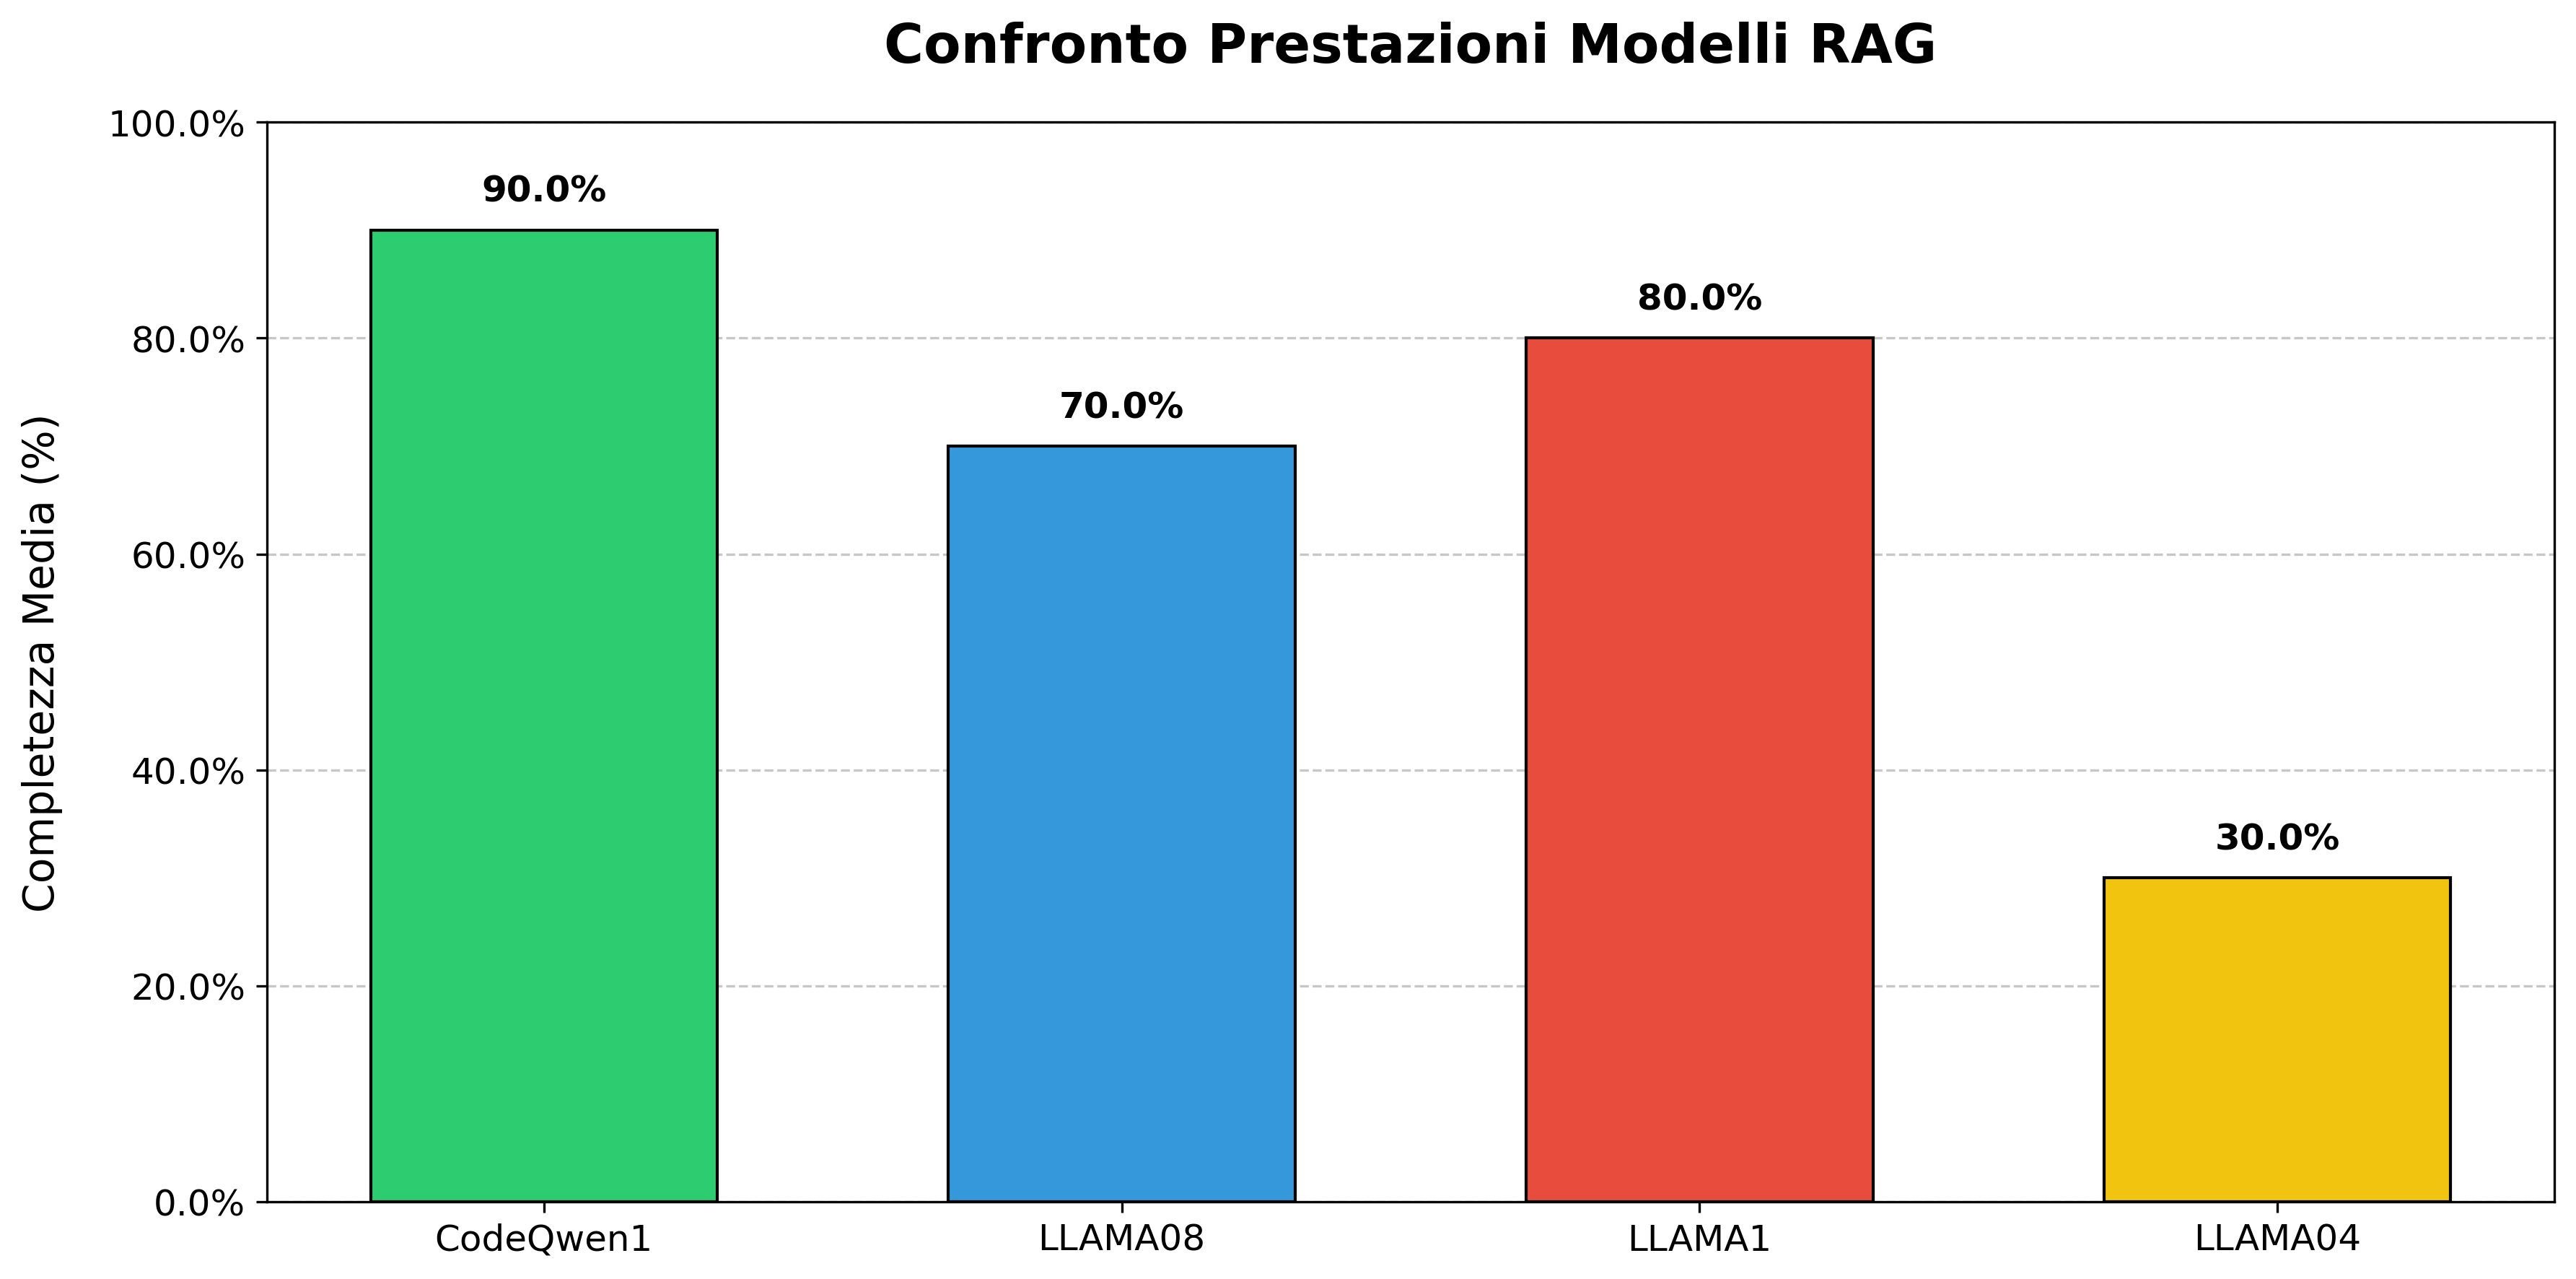
\includegraphics[width=\textwidth]{figures/confronto_valutazioni_modelli.png}
    \caption{Confronto risposte modelli RAG}
    \label{fig:confronto-modelli}
\end{figure}
\subsection{Analisi risultati}
La configurazione migliore è stata quella del LLM \textbf{CodeQwen con score threshold 1.0},
i test effettuati hanno dimostrato che è meglio aumentare la tolleranza di score dei chunk estratti nella fase di Retriever.
Questo score relativamente alto, come già analizzato nei capitoli precedenti, può causare l'inserimento di alcuni chunk non coerenti ma allo stesso tempo evita di escludere chunk validi e fondamentali per permettere al LLM di rispondere correttamente.
Quando il RAG trova i chunk corretti abbiamo dimostrato che score\_threshold ha valore molto basso solo nei casi in cui la query di input è scritta in maniera molto accurata cosa che 
normalmente non avviene.
Il risultato di questa minore rigidità nel filtrare i chunk può essere utile per ridurre l'overfitting creato nella prima fas di configurazione dei parametri dell RAG.
Per validare la soluzione adottata e prevenire il plorifirarsi di chunk non coerenti viene sempre impostato il limite a 5 Chunk.
In questo modo il Prompt non viene mai eccessivamente appesantito e il modello riesce ad elaborare nella maggior parte dei casi risposte coerenti.
I test fatti su Llma3.2 con score threshold 1.0 e con threshold 0.8 esplicitano queste conclusioni infatti il risultato migliore è stato con score\_threshold più altro perchè in questo modo 
non sono stati estromessi nella fase di Retriever chunk validi e fondamentali per la risposta.
I risultati sono stati nel complesso soddisfacenti ed è possibile concludere che il sistema RAG funziona correttamente aumentando le conoscenze dei LLM in modo vincente.
Ulteriore test è stato fatto impostando uno score\_threshold 0.4 con il quale vengono esclusi di fatto quasi tutti i chunck, in questo modo il LLM risponde solo utilizzando le sue con conoscenze riportando risultati estremamente scarsi non conoscendo i contesti e le librerie specificate nelle domande.
\begin{figure}[h]
    \centering
    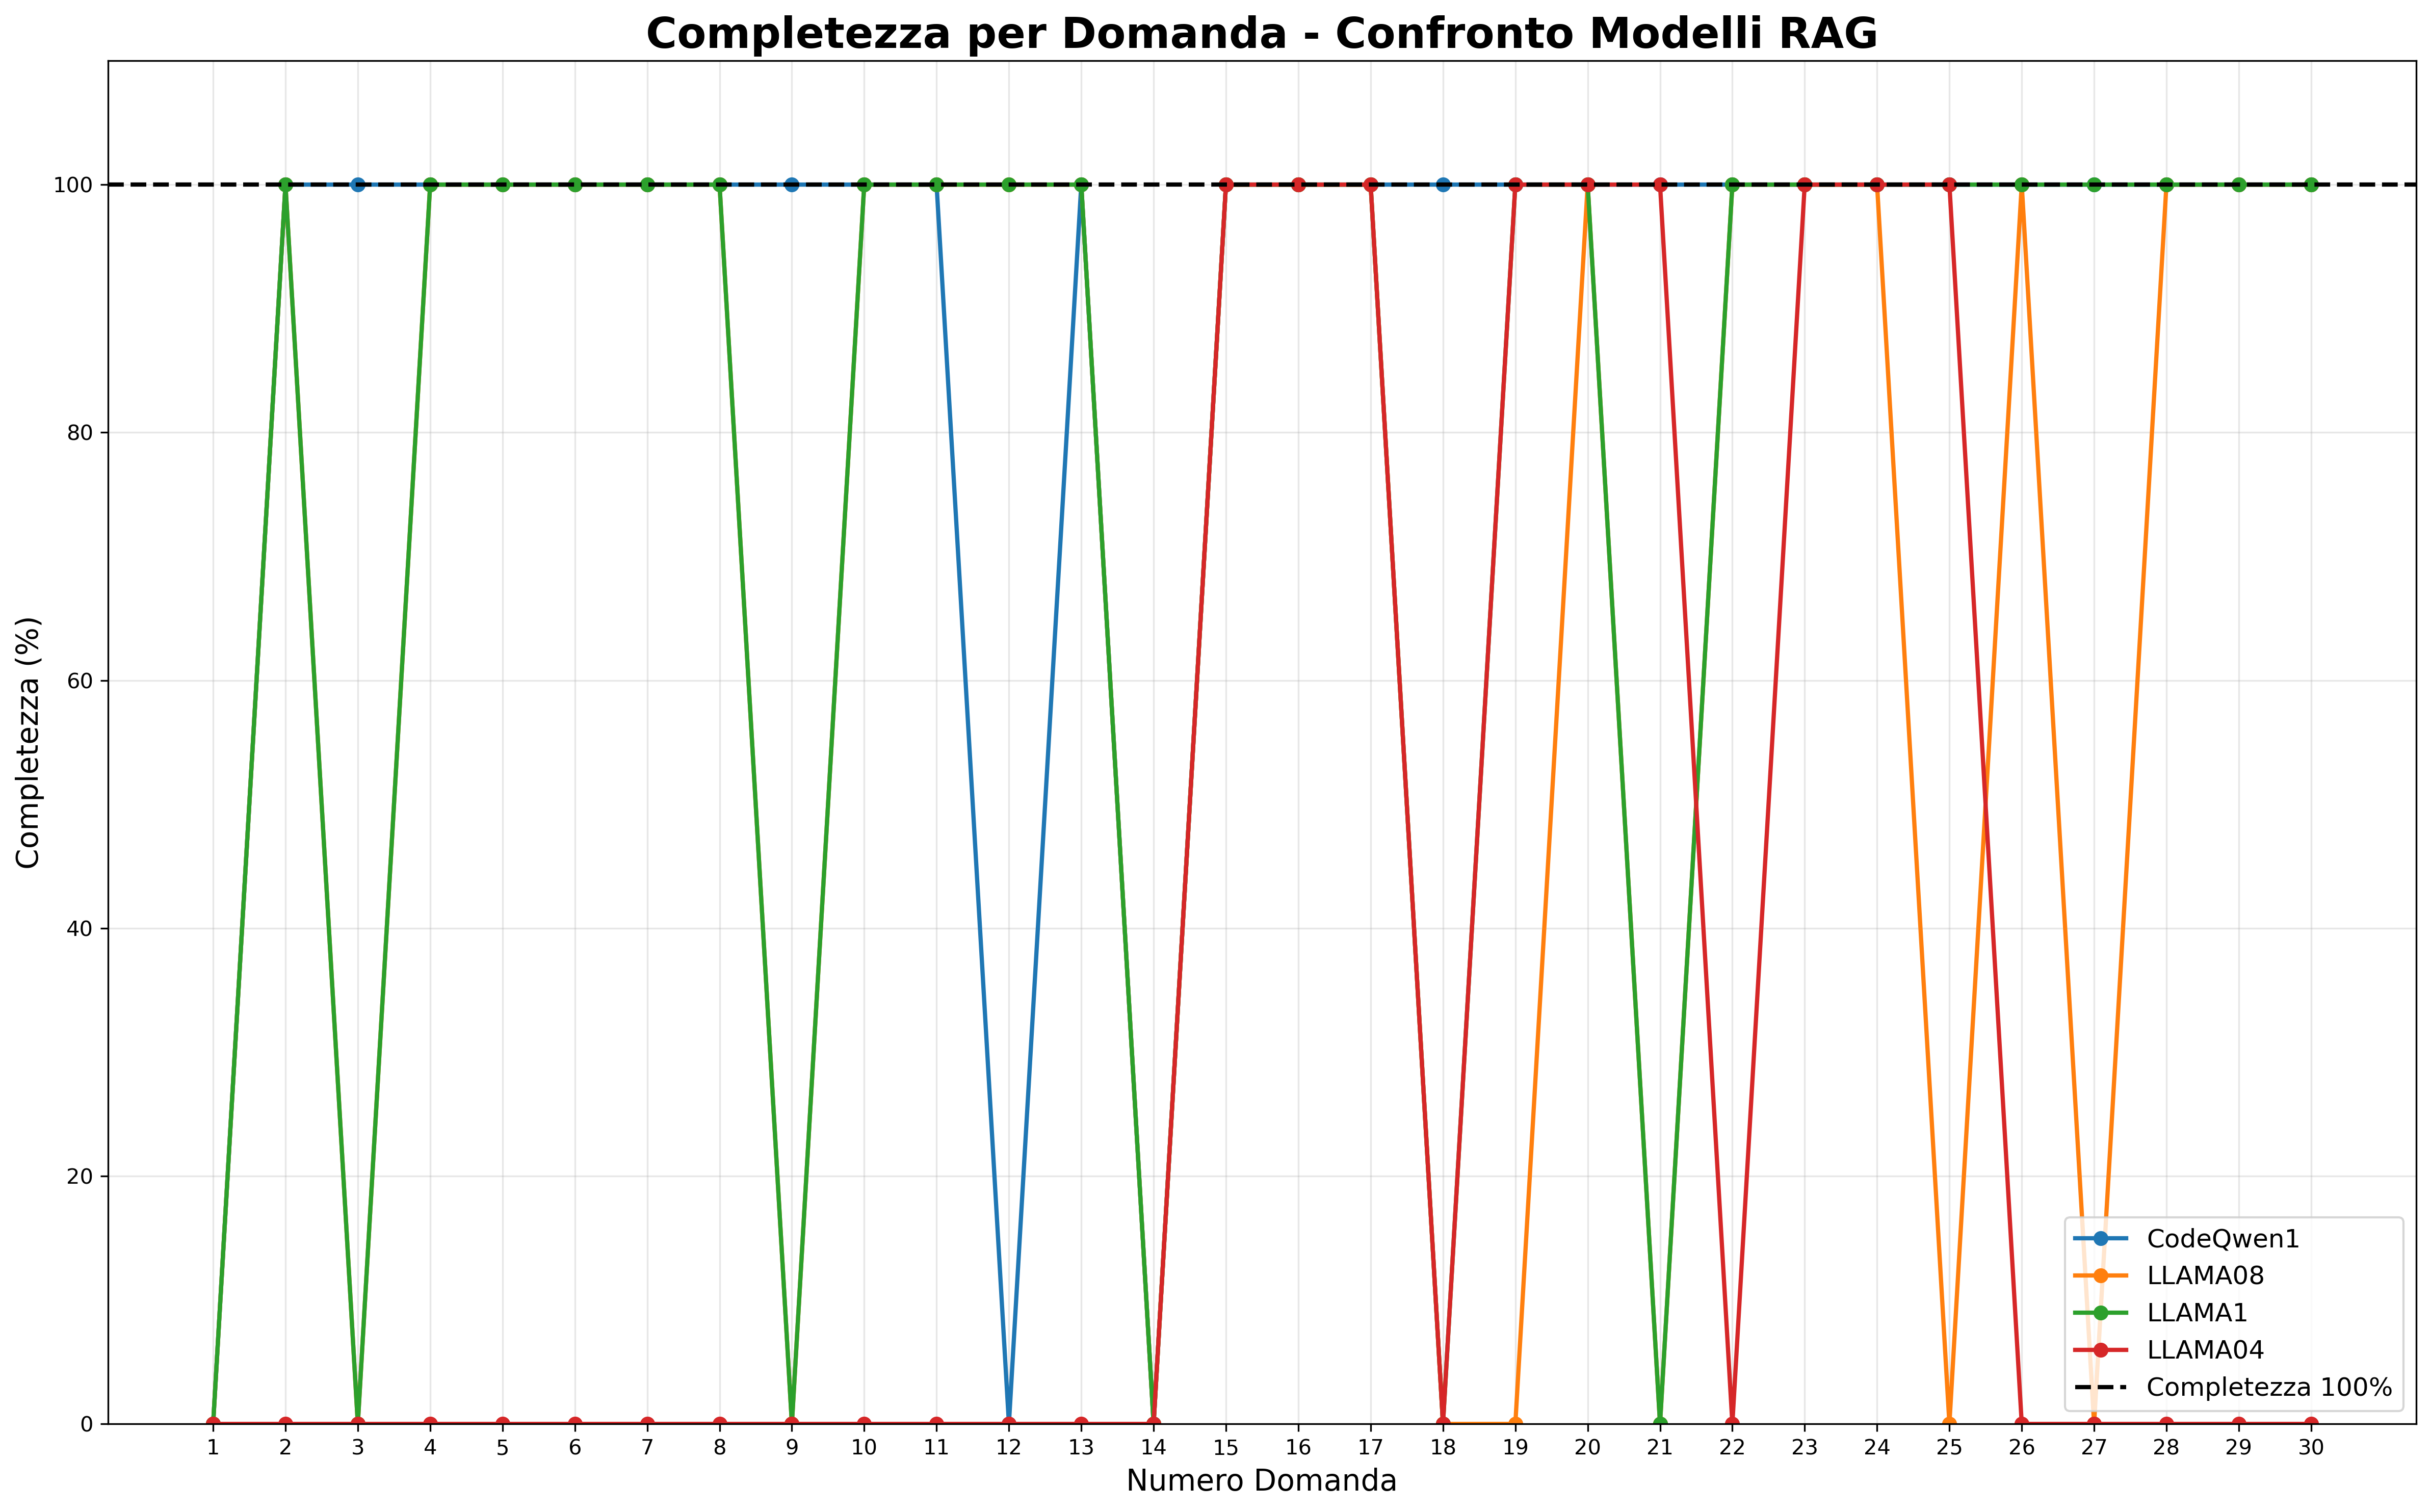
\includegraphics[width=\textwidth]{figures/completezza_per_domanda.png}
    \caption{Completezza per domanda}
    \label{fig:completezza-per-domanda}
\end{figure}

\paragraph{Nota:} È interessante ricordare che tutti i modelli hanno sbagliato la prima domanda,
non per mancanza di contesto nei chunk forniti al Prompt, ma come precedentemente descritto a causa di un errore nel calcolo del giorno della settimana.
Questo errore non si sarebbe verificato con le versioni con più parametri degli stessi modelli.

\chapter{Conclusioni}
\begin{quote}
    “Let an ultraintelligent machine be defined as a machine that can far surpass all the intellectual activities of any man however clever.
    Since the design of machines is one of these intellectual activities, an ultraintelligent machine could design even better machines; there would then unquestionably be an ‘intelligence explosion,’ and the intelligence of man would be left far behind.
    Thus the first ultraintelligent machine is the last invention that man need ever make.”
    
    \hfill--- \textit{I.J. Good (1965)\cite{Good1965}}
\end{quote}
\begin{figure}[h]
    \centering
    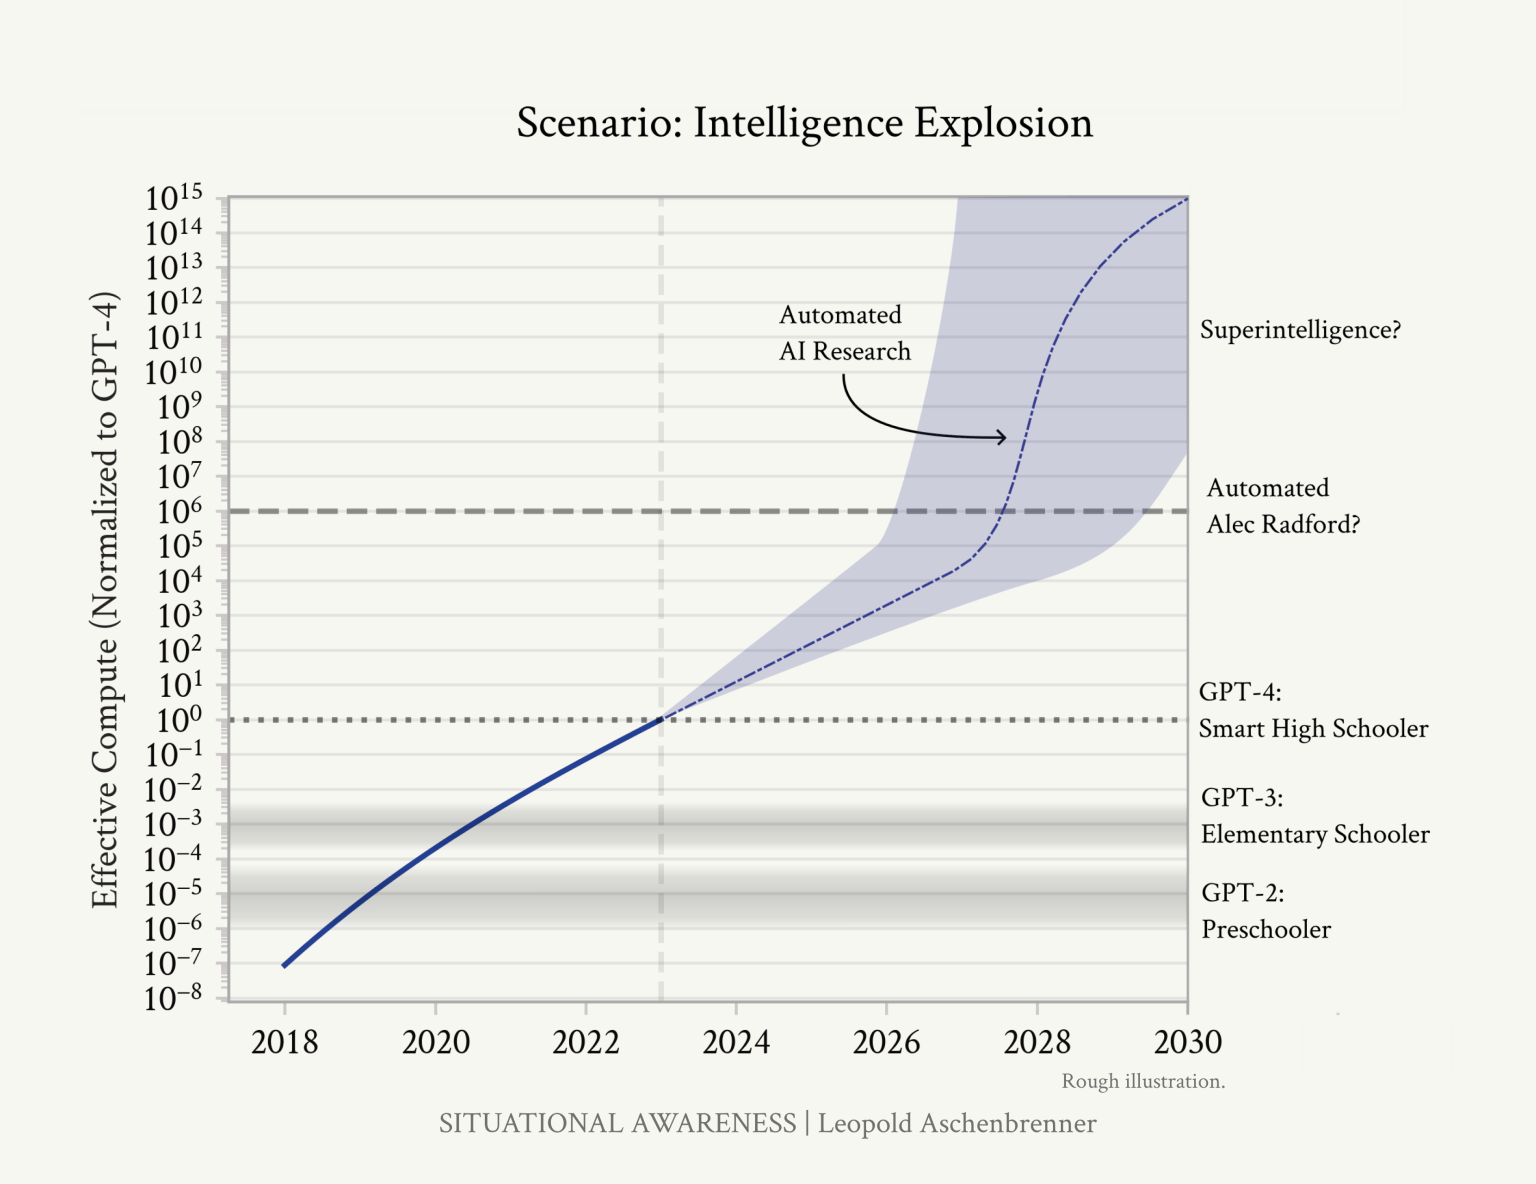
\includegraphics[width=\textwidth]{figures/intelligence_explosion.png}
    \caption{fig: tratta da situational-awareness.ai}
\end{figure}
Questi mesi di lavoro mi hanno portato a cercare di conosce e capire il più possibile come funzionano realmente i Large Language Model.
Nella fase di ricerca ho sempre trovato nei vari articoli e analisi stupore e meraviglia nel commentare i risultati e le capacità dimostrate da questi modelli.
Il saggio di Leopold Aschenbrenner \cite{Aschenbrenner2024} ``SITUATIONAL AWARENESS: The Decade Ahead'', da me inontrato quasi al termine della scrittura di questa tesi, spiega e approfondisce lo stesso giudizio che oggi ho sul futuro dell'Artificial intelligence.
Non voglio addentrarmi ora in ulteriori giudizi generali sul futuro dell'AI preferendo tornare nel contesto di questa tesi e affermere che \textbf{l'integrazione di RAG e LLM nello sviluppo del Software} è oggi già piena realtà.
Il sistema RAG d'esempio implementato funziona correttamente nonostante i limiti dei modelli utilizzati e con un ulteriore implementazione delle tecniche Chunking potrebbe essere realmente utilizzato a livello aziendale con buoni risultati.
Implementare sistemi RAG per le aziende oggi è un ottima soluzione,
ma resta sempre il peso e la consapevolezza che in questo momento, le soluzioni costruite, sono sempre un passo indietro rispetto ai miglioramenti globali che
giornalmente vengono rilasciati.
Come programmatore userò questi strumenti nel mio lavoro marginalmente perchè è mio desiderio continuare ad avere il controllo dei progetti realizzati che sento spesso di perdere utilizzando questi strumenti.
Altro motivo e per continuare ad avere soddisfazione e orgoglio nel trovare soluzioni in autonomia, 
certo sono consapevole che permettendo di velocizzare e migliorare la qualità del mio codice facendomi
conoscere e ragionare su nuove tecniche e soluzioni aumentando la mia base di conoscenza.
L'espressione \emph{``Se la ruota è già stata inventata, perchè reinventarla''} invita a non ripetere un lavoro già svolto con successo,
ma è anche vero che il codice è stato inventato e migliorato da tanti programmatori che hanno cercato di renderlo più adatta ai loro scopi.
Proprio per questo mi piace concludere pensando che noi programmatori (semplicemente) stiamo imparando da altri programmatori che non incontreremo e conosceremo mai di persona e l'AI sia, in questo campo, (solo) un grandissimo trasmettitore di conoscenza.

\begin{quote}
    “De nihilo nihil”
    \hfill--- \textit{Lucrezio (~55 a.c) }
\end{quote}

\chapter{Ringraziamenti}
Ringrazio il mio relatore il Prof. Viroli Mirko e il Dott. Aguzzi Gianluca per l'interessantissimo argomento di tesi proposto e per la disponibilità e professionalità dimostrata.
Ringrazio tutta lo comunità di ricercatori che forniscono materiale open source e documentazione per permettere a tutti di apprendere e migliorare questa incredibile tecnologia.
Grazie a tutti gli studenti che ho conosciuto in questo percorso, è stato molto costruttivo e divertente studiare con voi.
Infine vorrei trovare le parole giuste per ringraziare Giulia, in questi anni sei stata eccezzionale grazie per tutto, questo risultato è in gran parte merito tuo.





%----------------------------------------------------------------------------------------
% BIBLIOGRAPHY
%----------------------------------------------------------------------------------------

\backmatter

\nocite{*} % Remove this as soon as you have the first citation

\bibliographystyle{alphaurl}
%\bibliographystyle{plainurl}
\bibliography{bibliography}

\end{document}
